\documentclass[12pt,a4paper]{report}

% ==============================================================================
% CÁC GÓI THƯ VIỆN CẦN THIẾT
% ==============================================================================
\usepackage[utf8]{vietnam}
\usepackage[top=2.5cm,bottom=2.5cm,left=3cm,right=2cm,headheight=15pt]{geometry}
\usepackage{graphicx}
\usepackage{amsmath,amssymb}
\usepackage{booktabs}
\usepackage{array}
\usepackage{longtable}
\usepackage{enumitem}
\usepackage{xcolor}
\usepackage{colortbl}
\usepackage{listings}
\usepackage{tikz}
\usetikzlibrary{calc, shapes.geometric, shapes.multipart, arrows.meta, positioning}
\usepackage{fancyhdr}
\usepackage{tabularx}
\newcolumntype{L}[1]{>{\raggedright\arraybackslash}p{#1}}
\newcolumntype{Y}{>{\raggedright\arraybackslash}X}
\usepackage{float}
\usepackage{titlesec}
\usepackage[unicode,colorlinks=true,linkcolor=black,citecolor=blue,urlcolor=blue]{hyperref}

% Cấu hình hiển thị code (listings)
\definecolor{codegreen}{rgb}{0,0.6,0}
\definecolor{codegray}{rgb}{0.5,0.5,0.5}
\definecolor{codepurple}{rgb}{0.58,0,0.82}
\definecolor{backcolour}{rgb}{0.96,0.96,0.96}

% Màu sắc cho sơ đồ ERD
\definecolor{erdblue}{RGB}{20, 60, 110}
\definecolor{erdbg}{RGB}{250, 251, 253}
\definecolor{pkcolor}{RGB}{180, 20, 20}
\definecolor{fkcolor}{RGB}{15, 125, 45}
\definecolor{uqcolor}{RGB}{200, 100, 0}
\definecolor{typecolor}{RGB}{90, 100, 115}

\lstdefinestyle{mystyle}{
    backgroundcolor=\color{backcolour},   
    commentstyle=\color{codegreen},
    keywordstyle=\color{blue}\bfseries,
    numberstyle=\tiny\color{codegray},
    stringstyle=\color{codepurple},
    basicstyle=\ttfamily\footnotesize,
    breakatwhitespace=false,         
    breaklines=true,                 
    captionpos=b,                    
    keepspaces=true,                 
    numbers=left,                    
    numbersep=5pt,                  
    showspaces=false,                
    showstringspaces=false,
    showtabs=false,                  
    tabsize=2,
    frame=single,
    rulecolor=\color{codegray}
}
\lstset{style=mystyle}

% Cấu hình header & footer
\pagestyle{fancy}
\fancyhf{}
\fancyhead[L]{\small Báo cáo BTL: Hệ Quản trị Cơ sở Dữ liệu}
\fancyhead[R]{\small Nhóm 11 -- Đề tài A2}
\fancyfoot[C]{\thepage}
\renewcommand{\headrulewidth}{0.4pt}
\renewcommand{\footrulewidth}{0.4pt}

% ==============================================================================
% BẮT ĐẦU TÀI LIỆU
% ==============================================================================
\begin{document}

% ------------------------------------------------------------------------------
% TRANG BÌA (Cover Page)
% ------------------------------------------------------------------------------
\begin{titlepage}
\thispagestyle{empty}
\hypersetup{pageanchor=false}
\begin{tikzpicture}[remember picture, overlay]
  % Khung viền kép ngoài (dày) và trong (mảnh) chuẩn mẫu UET
  \draw[line width=1.6pt] ($(current page.north west) + (2cm,-2cm)$) rectangle ($(current page.south east) + (-1.5cm,2cm)$);
  \draw[line width=0.6pt] ($(current page.north west) + (2.12cm,-2.12cm)$) rectangle ($(current page.south east) + (-1.62cm,2.12cm)$);
\end{tikzpicture}

\begin{center}
    \vspace*{0.2cm}
    {\large \textbf{ĐẠI HỌC QUỐC GIA HÀ NỘI}}\\[0.15cm]
    {\large \textbf{TRƯỜNG ĐẠI HỌC CÔNG NGHỆ}}\\[0.25cm]
    \rule{5.2cm}{0.8pt}\\[0.8cm]

    % Logo trường do sinh viên chuẩn bị
    
\includegraphics[width=3.2cm]{images/uet_logo.png}\\[0.9cm]

    {\Large \textbf{BÁO CÁO BÀI TẬP LỚN}}\\[0.3cm]
    {\large \textbf{MÔN: HỆ QUẢN TRỊ CƠ SỞ DỮ LIỆU}}\\[0.15cm]
    {\large \textbf{MÃ LỚP HỌC PHẦN: INT3202 3}}\\[0.9cm]

    {\large \textbf{ĐỀ TÀI A2:}}\\[0.35cm]
    {\large \textbf{THIẾT LẬP NHÂN BẢN 1 MASTER, 2 SLAVE;}}\\[0.25cm]
    {\large \textbf{ÁP DỤNG THỬ NGHIỆM VỚI CSDL}}\\[0.25cm]
    {\large \textbf{QUẢN LÝ BÁN HÀNG TẠI 1 SIÊU THỊ}}\\[1.3cm]

    \begin{minipage}{0.85\textwidth}
        \begin{tabular}{@{}p{5.8cm}l@{}}
            \textbf{Giảng viên hướng dẫn:} & GVC. ThS. Vũ Bá Duy \\[0.4cm]
            \textbf{Nhóm sinh viên thực hiện:} & Nhóm 11 \\[0.25cm]
            1. Lê Bá Sơn (Nhóm trưởng) & MSSV: 24020294 \\[0.15cm]
            2. Lê Bá Minh Hiếu & MSSV: 24020125 \\[0.15cm]
            3. Nguyễn Văn Tiến & MSSV: 24020321 \\
        \end{tabular}
    \end{minipage}

    \vfill
    {\large \textbf{HÀ NỘI -- 2026}}\\[0.2cm]
\end{center}
\end{titlepage}

\hypersetup{pageanchor=true}

% ------------------------------------------------------------------------------
% LỜI MỞ ĐẦU & PHÂN CÔNG NHIỆM VỤ
% ------------------------------------------------------------------------------
\pagenumbering{roman}
\chapter*{Lời Mở Đầu}
\addcontentsline{toc}{chapter}{Lời Mở Đầu}

Trong bối cảnh bùng nổ chuyển đổi số và thương mại bán lẻ hiện đại, các chuỗi siêu thị phải đối mặt với hàng chục nghìn giao dịch mua bán, thanh toán mỗi ngày. Việc chỉ sử dụng một máy chủ cơ sở dữ liệu tập trung duy nhất bộc lộ rất nhiều nguy cơ: quá tải khi quét mã vạch giờ cao điểm, nguy cơ mất trắng dữ liệu khi phần cứng sập nguồn đột ngột (Single Point of Failure -- SPOF), và không thể mở rộng hiệu năng truy xuất theo chiều ngang.

Để giải quyết bài toán này, kỹ thuật nhân bản theo kiến trúc \mbox{\textbf{Master -- Slave}} là một trong những giải pháp được áp dụng rộng rãi. Với quy mô của một siêu thị, cấu hình \mbox{\textbf{1 Master -- 2 Slaves}} được lựa chọn nhằm cân bằng giữa chi phí hạ tầng và hiệu năng vận hành: nút Master chuyên tiếp nhận các giao dịch ghi (xuất hóa đơn, trừ kho), trong khi hai nút Slave đóng vai trò bản sao chỉ đọc (\textit{Read-only}) giúp phân tải truy vấn cho hàng chục quầy thu ngân, đồng thời lưu giữ bản sao dự phòng để phục vụ chuyển đổi thay thế khi máy chủ chính gặp sự cố.

Báo cáo bài tập lớn này được thực hiện trong khuôn khổ học phần Hệ Quản trị Cơ sở Dữ liệu, tập trung vào giai đoạn triển khai thực nghiệm của đề tài A2: Thiết lập nhân bản 1 Master, 2 Slave; áp dụng thử nghiệm với CSDL quản lý bán hàng tại 1 siêu thị. Trọng tâm của báo cáo là xây dựng mô hình cụm cơ sở dữ liệu phân tán hoàn chỉnh, đánh giá khả năng phân tải truy vấn đọc -- ghi và kiểm chứng tính sẵn sàng, độ tin cậy của hệ thống trước các kịch bản sự cố thực tế.

Nhóm chúng em xin chân thành cảm ơn thầy \textbf{GVC. ThS. Vũ Bá Duy} đã tận tình hướng dẫn, trang bị những nền tảng lý thuyết phân tán vững chắc để nhóm có thể triển khai hệ thống thực nghiệm này.

\vspace{1cm}
\noindent \textbf{Bảng phân công nhiệm vụ của từng thành viên trong nhóm:}

\begin{table}[h!]
\centering
\begin{tabular}{|c|l|c|p{7.5cm}|}
\hline
\textbf{STT} & \textbf{Họ và tên} & \textbf{Mã SV} & \textbf{Nội dung phụ trách chính} \\ \hline
1 & Lê Bá Sơn & 24020294 & Thiết kế kiến trúc cụm Docker, xây dựng CSDL siêu thị, kịch bản DML xuôi và cấu hình GTID. \\ \hline
2 & Lê Bá Minh Hiếu & 24020125 & Thiết lập cơ chế Super Read-Only, kiểm thử tính toàn vẹn Transaction và đo đạc độ trễ . \\ \hline
3 & Nguyễn Văn Tiến & 24020321 & Triển khai kịch bản chịu lỗi, Online DDL và kịch bản thảm họa Failover. \\ \hline
\end{tabular}
\end{table}

\newpage

% ------------------------------------------------------------------------------
% MỤC LỤC & DANH MỤC
% ------------------------------------------------------------------------------
\tableofcontents
\newpage
\newpage

\pagenumbering{arabic}

% ------------------------------------------------------------------------------
% CHƯƠNG 1
% ------------------------------------------------------------------------------
\chapter{Tổng Quan Và Thiết Kế Kiến Trúc Cụm Nhân Bản}

\section{Đặt Vấn Đề và Thách Thức trong Quản Lý CSDL Siêu Thị}

\subsection{Hạn chế của mô hình CSDL Tập trung truyền thống}
Trong các hệ thống chuỗi siêu thị bán lẻ hiện đại, hệ thống cơ sở dữ liệu phải xử lý liên tục hàng chục nghìn lượt giao dịch mỗi ngày. Khi sử dụng một máy chủ CSDL đơn lẻ, hệ thống nhanh chóng đối mặt với ba rào cản kỹ thuật nghiêm trọng:
\begin{enumerate}
    \item \textbf{Tắc nghẽn I/O và suy giảm hiệu năng tại giờ cao điểm:} Tại các khung giờ cao điểm (cuối tuần, lễ Tết), hàng chục quầy thu ngân thực hiện quét mã vạch tra cứu giá, áp mã khuyến mãi và thanh toán đồng thời. Các thao tác đọc và ghi cạnh tranh trực tiếp tài nguyên đĩa cứng và khóa, gây nghẽn hàng đợi và làm chậm toàn bộ hệ thống.
    \item \textbf{Rủi ro đơn điểm lỗi (Single Point of Failure -- SPOF):} Khi toàn bộ dữ liệu chỉ nằm trên một máy chủ duy nhất, bất kỳ sự cố phần cứng nào (cháy nguồn, hỏng ổ cứng, đứt cáp mạng) cũng sẽ làm tê liệt toàn bộ hoạt động thanh toán của siêu thị, gây ảnh hưởng đáng kể về kinh tế và trải nghiệm khách hàng.
    \item \textbf{Giới hạn của mở rộng theo chiều dọc:} Để tăng năng lực xử lý, giải pháp nâng cấp phần cứng thường tốn kém chi phí và nhanh chóng chạm trần giới hạn vật lý của bo mạch chủ mà không giải quyết được tính sẵn sàng cao.
\end{enumerate}

\subsection{Nhu cầu phân tách Đọc -- Ghi đặc thù của ngành bán lẻ}
Khảo sát thực tế trong hoạt động siêu thị cho thấy tỷ lệ truy xuất dữ liệu có sự chênh lệch rõ rệt giữa hai luồng:
\begin{itemize}
    \item \textbf{Luồng Đọc:} Bao gồm các thao tác quét mã vạch kiểm tra thông tin mặt hàng, tra cứu tồn kho, kiểm tra điểm tích lũy thành viên, xuất báo cáo doanh thu theo ca.
    \item \textbf{Luồng Ghi:} Chỉ phát sinh khi khách hàng hoàn tất thanh toán và in hóa đơn hoặc thủ kho nhập thêm hàng mới.
\end{itemize}

Xuất phát từ nhu cầu đọc vượt trội, giải pháp phù hợp là phân tách độc lập luồng Đọc và Ghi thông qua mô hình nhân bản \textbf{1 Master -- 2 Slave}: Master tập trung tài nguyên cho các giao dịch ghi cốt lõi, trong khi 2 Slave chia sẻ tải đọc của hàng chục quầy thu ngân.

\begin{table}[htbp]
\centering
\caption{So sánh Kiến trúc CSDL Tập trung và Cụm Nhân bản}
\label{tab:ss_kientruc}
\begin{tabularx}{\linewidth}{|>{\raggedright\arraybackslash\bfseries}p{4.2cm}|>{\raggedright\arraybackslash}X|>{\raggedright\arraybackslash}X|}
\hline
\textmd{\textbf{Tiêu chí}} & \textmd{\textbf{CSDL Tập trung}} & \textmd{\textbf{Cụm Nhân bản}} \\ \hline
Tính sẵn sàng & Thấp; gián đoạn hoạt động khi máy chủ gặp sự cố. & Rất cao; hỗ trợ thay thế khi Master gặp lỗi. \\ \hline
Hiệu năng đọc & Nghẽn I/O đĩa khi lượng truy vấn đọc/ghi tăng cao. & Tăng mạnh nhờ cơ chế phân tải đọc sang các trạm Slave. \\ \hline
Khả năng mở rộng & Mở rộng chiều dọc tốn kém và có giới hạn vật lý. & Mở rộng chiều ngang linh hoạt khi cần nâng công suất. \\ \hline
Bảo vệ dữ liệu & Rủi ro mất mát dữ liệu nếu phát sinh hỏng hóc phần cứng. & Dữ liệu được nhân bản bất đồng bộ liên tục sang các trạm bản sao dự phòng. \\ \hline
Chi phí triển khai & Yêu cầu máy chủ cấu hình lớn, chi phí đầu tư cao. & Tối ưu chi phí nhờ tận dụng các máy chủ phổ thông kết nối nội bộ. \\ \hline
\end{tabularx}
\end{table}

\section{Nguyên Lý Hoạt Động của Nhân Bản Dữ Liệu}

\subsection{Bản chất của kỹ thuật Nhân bản mức Logic}
Hệ quản trị CSDL MySQL sử dụng cơ chế nhân bản mức sự kiện logic thay vì sao chép từng khối đĩa cứng vật lý. Nhờ đó, các máy Slave vừa duy trì tiếp nhận thay đổi vừa có thể mở cửa cho hàng nghìn quầy thu ngân đọc dữ liệu đồng thời.

\subsection{Kiến trúc luồng và chu trình nhân bản bất đồng bộ}
Quá trình nhân bản giữa Master và các Slave diễn ra liên tục qua 3 luồng xử lý ngầm độc lập:
\begin{enumerate}
    \item \textbf{Luồng Binlog Dump Thread (trên Master):} Khi Slave kết nối đến Master, Master sinh ra một luồng Dump Thread chuyên dụng. Luồng này liên tục đọc các sự kiện mới trong Binary Log của Master và truyền trực tiếp qua kết nối mạng TCP/IP socket sang Slave.
    \item \textbf{Luồng Receiver / IO Thread (trên Slave):} Luồng này lắng nghe các gói tin gửi từ Master, tiếp nhận các sự kiện nhị phân và ghi tuần tự vào một tệp nhật ký cục bộ trên Slave gọi là Relay Log.
    \item \textbf{Luồng Applier / SQL Thread (trên Slave):} Độc lập với luồng IO, luồng SQL liên tục đọc các sự kiện từ Relay Log, giải mã và thực thi lại y hệt các câu lệnh đó vào động cơ lưu trữ InnoDB của Slave, đưa dữ liệu của Slave đồng nhất với Master.
\end{enumerate}

Mô hình tách biệt ba luồng trên vận hành theo cơ chế \textbf{nhân bản bất đồng bộ}: ngay khi Master ghi nhận xong giao dịch xuống nhật ký của chính nó và thực hiện \texttt{COMMIT}, Master lập tức chuyển sang xử lý giao dịch tiếp theo mà không phải đứng chờ xác nhận từ các Slave. Cơ chế này đặc biệt phù hợp với nghiệp vụ bán lẻ siêu thị vì giữ cho quầy thu ngân luôn thanh toán tức tốc và không bị treo dây chuyền nếu một máy Slave gặp sự cố mạng; các thay đổi được truyền ngầm sang Slave chỉ sau vài mili-giây và được khóa chỉ đọc bảo vệ khỏi xung đột dữ liệu.

\begin{figure}[htbp]
\centering
\resizebox{\linewidth}{!}{%
\begin{tikzpicture}[
    box/.style={rectangle, draw=blue!75!black, fill=blue!6, rounded corners=5pt, line width=1.3pt, align=center, minimum width=4.8cm, minimum height=1.05cm, font=\small},
    storage/.style={rectangle, draw=purple!80!black, fill=purple!6, rounded corners=5pt, line width=1.3pt, align=center, minimum width=4.8cm, minimum height=1.05cm, font=\small},
    thread/.style={rectangle, draw=orange!90!black, fill=orange!12, rounded corners=12pt, line width=1.3pt, align=center, minimum width=4.8cm, minimum height=1.05cm, font=\small\bfseries},
    client/.style={rectangle, draw=teal!80!black, fill=teal!6, rounded corners=5pt, line width=1.3pt, align=center, minimum width=4.8cm, minimum height=1.05cm, font=\small},
    netbox/.style={rectangle, draw=red!75!black, fill=red!8, rounded corners=6pt, line width=1.3pt, align=center, font=\small\bfseries, text=red!85!black, minimum width=2.8cm, minimum height=1.05cm},
    arrow_m/.style={draw=blue!85!black, -{Stealth[length=4.5mm, width=3.2mm]}, line width=2.0pt},
    arrow_s/.style={draw=green!55!black, -{Stealth[length=4.5mm, width=3.2mm]}, line width=2.0pt},
    arrow_net/.style={draw=red!80!black, -{Stealth[length=4.5mm, width=3.2mm]}, line width=2.2pt},
    lbl_m/.style={font=\footnotesize\bfseries, text=blue!85!black, anchor=west},
    lbl_s/.style={font=\footnotesize\bfseries, text=green!50!black, anchor=west}
]
    % ================= KHUNG MASTER =================
    \node [anchor=south, font=\bfseries\large, text=blue!85!black] at (0, 7.9) {MÁY CHỦ MASTER (Port 3306)};
    \node [client] (app_write) at (0, 7.1) {\textbf{Ứng dụng Bán hàng}\\(Giao dịch Ghi)};

    % Container Master
    \draw [dashed, line width=1.2pt, draw=blue!70, fill=blue!2] (-3.8, -0.4) rectangle (3.8, 5.4);

    \node [box] (master_db) at (0, 4.5) {\textbf{InnoDB Storage Engine}\\(Dữ liệu gốc Master)};
    \node [storage] (binlog) at (0, 2.45) {\textbf{Binary Log}\\(\texttt{mysql-bin.00000x})};
    \node [thread] (dump_thread) at (0, 0.4) {Binlog Dump Thread};

    % ================= KHUNG SLAVE =================
    \node [anchor=south, font=\bfseries\large, text=green!55!black] at (12.6, 7.9) {MÁY CHỦ SLAVE 1 \& 2 (Port 3307/3308)};
    \node [client] (app_read) at (12.6, 7.1) {\textbf{Quầy Thu ngân / Báo cáo}\\(Truy vấn Đọc)};

    % Container Slave
    \draw [dashed, line width=1.2pt, draw=green!60!black, fill=green!2] (8.8, -0.4) rectangle (16.4, 5.4);

    \node [box] (slave_db) at (12.6, 4.5) {\textbf{InnoDB Storage Engine}\\(Super Read-Only)};
    \node [storage] (relay_log) at (12.6, 2.45) {\textbf{Relay Log \& SQL Applier}\\(\texttt{mysql-relay-bin.00000x})};
    \node [thread] (io_thread) at (12.6, 0.4) {Replica I/O Thread};

    % ================= MẠNG DOCKER =================
    \node [netbox] (net) at (6.3, 0.4) {Mạng Docker\\(\texttt{dbms-net})};

    % ================= MŨI TÊN MASTER (ĐI XUỐNG) =================
    \draw [arrow_m] (0, 6.575) -- (0, 5.025);
    \node [lbl_m] at (0.3, 5.95) {(1) Ghi dữ liệu};

    \draw [arrow_m] (0, 3.975) -- (0, 2.975);
    \node [lbl_m] at (0.3, 3.475) {(2) Ghi binlog};

    \draw [arrow_m] (0, 1.925) -- (0, 0.925);
    \node [lbl_m] at (0.3, 1.425) {(3) Đọc sự kiện};

    % ================= MŨI TÊN MẠNG (NGANG) =================
    \draw [arrow_net] (dump_thread.east) -- (net.west);
    \draw [arrow_net] (net.east) -- (io_thread.west);
    \node [above=6pt, font=\footnotesize\bfseries, text=red!80!black] at (6.3, 0.95) {(4) Gói tin mạng TCP/IP};

    % ================= MŨI TÊN SLAVE (ĐI LÊN) =================
    \draw [arrow_s] (12.6, 0.925) -- (12.6, 1.925);
    \node [lbl_s] at (12.9, 1.425) {(5) Ghi tiếp sức};

    \draw [arrow_s] (12.6, 2.975) -- (12.6, 3.975);
    \node [lbl_s] at (12.9, 3.475) {(6) Thực thi SQL};

    \draw [arrow_s] (12.6, 5.025) -- (12.6, 6.575);
    \node [lbl_s] at (12.9, 5.95) {(7) Phục vụ đọc};

\end{tikzpicture}%
}
\caption{Kiến trúc luồng truyền dữ liệu và chu trình nhân bản logic trong MySQL}
\label{fig:replication_threads}
\end{figure}

\section{Thiết Kế Kiến Trúc Cụm 1 Master -- 2 Slave trên Docker}

\subsection{Mô hình Ảo hóa và Mạng Liên lạc Nội bộ}
Hệ thống cụm cơ sở dữ liệu phân tán được ảo hóa hoàn toàn bằng công nghệ container Docker và điều phối tập trung thông qua tệp cấu hình \texttt{docker-compose.yml}. Cả 3 node đều khởi chạy phiên bản MySQL 8.0 ổn định, cùng tham gia vào một mạng ảo hóa độc lập:
\begin{itemize}
    \item \textbf{Mạng ảo hóa cô lập (\texttt{dbms-net}):} Nhóm cấu hình một mạng bridge chuyên dụng mang tên \texttt{dbms-net}. Mạng này thiết lập một phân vùng mạng con ảo tách biệt hoàn toàn với môi trường máy chủ host, ngăn chặn các truy cập trái phép từ bên ngoài quét thẳng vào các cổng dịch vụ nội bộ của CSDL.
    \item \textbf{Cơ chế phân giải tên miền nhúng:} Docker Engine tích hợp sẵn một máy chủ DNS nội bộ phục vụ riêng cho mạng bridge. Các container trong cụm liên lạc với nhau trực tiếp qua định danh dịch vụ (\texttt{mysql-master}, \texttt{mysql-slave-1}, \texttt{mysql-slave-2}). Cơ chế này đóng vai trò quan trọng trong kiến trúc nhân bản: khi một container gặp sự cố và khởi động lại, địa chỉ IP động có thể bị thay đổi, nhưng luồng kết nối nhân bản giữa các node vẫn duy trì liên tục và chuẩn xác nhờ phân giải tự động theo tên dịch vụ mà không cần tái cấu hình IP thủ công.
\end{itemize}

\subsection{Cơ chế Quản lý Lưu trữ Bền vững}
Do đặc thù các container là môi trường vô trạng thái và dữ liệu bên trong lớp ghi sẽ bị xóa sạch khi container bị hủy hoặc tái tạo, nhóm đã thiết lập giải pháp lưu trữ bền vững thông qua Docker Volume:
\begin{itemize}
    \item \textbf{Khởi tạo Volume định danh độc lập:} Ba ổ đĩa ảo riêng biệt được định nghĩa trong \texttt{docker-compose.yml} gồm \texttt{master\_data}, \texttt{slave1\_data} và \texttt{slave2\_data}. Mỗi volume được gắn kết vào thư mục \texttt{/var/lib/mysql} chứa dữ liệu cốt lõi của từng container tương ứng.
    \item \textbf{Bảo toàn dữ liệu và phân tách lưu trữ:} Việc sử dụng các volume riêng biệt đảm bảo rằng toàn bộ các tệp dữ liệu bảng InnoDB, Binary Log, Relay Log và trạng thái giao dịch GTID đều được lưu cố định trên hệ thống tệp của máy chủ host. Nhờ vậy, dữ liệu của cụm siêu thị được lưu giữ ổn định qua các chu kỳ khởi động lại, bảo trì hoặc nâng cấp container mà không xảy ra xung đột đọc/ghi tệp giữa các trạm.
\end{itemize}

\subsection{Phân định Vai trò và Quy hoạch Cổng Truy cập Ứng dụng}
Nhằm hiện thực hóa chiến lược phân tách tải Đọc -- Ghi cho ứng dụng quản lý bán hàng siêu thị, các nút trong cụm được phân công vai trò rõ ràng và ánh xạ cổng ra máy chủ host như sau:
\begin{itemize}
    \item \textbf{Phân luồng Ghi tại cổng 3306:} Cổng 3306 của máy host được kết nối trực tiếp đến \texttt{mysql-master}. Đây là cổng độc quyền phục vụ các giao dịch ghi từ quầy thu ngân và nhân viên quản trị.
    \item \textbf{Phân tải Đọc song song tại cổng 3307 và 3308:} Hai trạm Slave \texttt{mysql-slave-1} và \texttt{mysql-slave-2} được ánh xạ lần lượt ra cổng 3307 và 3308 của host. Các cổng này được sử dụng để cân bằng tải đọc, phục vụ hàng chục nhân viên thu ngân quét mã tra cứu sản phẩm và bộ phận kế toán xuất báo cáo tài chính mà không ảnh hưởng đến tiến trình thanh toán trên Master.
    \item \textbf{Chuỗi khởi động phụ thuộc:} Hai máy Slave được thiết lập ràng buộc phụ thuộc vào \texttt{mysql-master}, đảm bảo Master luôn được khởi tạo và sẵn sàng tiếp nhận luồng dữ liệu trước khi các luồng I/O Thread trên Slave tiến hành bắt tay đồng bộ.
\end{itemize}

\begin{table}[H]
\centering
\caption{Bảng thông số kỹ thuật cấu hình cụ thể của 3 node trong cụm}
\label{tab:cluster_specs}
\begin{tabularx}{\linewidth}{|>{\raggedright\arraybackslash}p{3.1cm}|>{\centering\arraybackslash}p{1.6cm}|>{\centering\arraybackslash}p{3.4cm}|>{\centering\arraybackslash}p{1.4cm}|>{\raggedright\arraybackslash}X|}
\hline
\textbf{Tên Container} & \textbf{Port Host} & \textbf{Port Container} & \textbf{Server ID} & \textbf{Vai trò và Chế độ hoạt động} \\ \hline
\texttt{mysql-master} & 3306 & 3306 & 1 &  Read/Write, ghi Binary Log, phân phối sự kiện đồng bộ. \\ \hline
\texttt{mysql-slave-1} & 3307 & 3306 & 2 &  Super Read-only, đệm Relay Log, sẵn sàng thay thế khi Master gặp sự cố. \\ \hline
\texttt{mysql-slave-2} & 3308 & 3306 & 3 &  Super Read-only, đệm Relay Log, chia sẻ tải đọc cho quầy thu ngân POS. \\ \hline
\end{tabularx}
\end{table}

\subsection{Phạm vi Môi trường Thực nghiệm và Lưu ý khi Triển khai Vật lý}
Cần lưu ý rằng trong phạm vi bài tập lớn, việc vận hành cả ba container trên cùng một máy chủ cá nhân đóng vai trò như một môi trường thử nghiệm có kiểm soát nhằm loại bỏ nhiễu đường truyền ngoại cảnh. Dù ba nút tách biệt về không gian mạng TCP/IP, tiến trình và ổ đĩa Volume để kiểm chứng đúng cơ chế GTID, khóa ghi hay Failover của MySQL, chúng vẫn chia sẻ chung CPU, RAM, băng thông đĩa cứng và nguồn điện của máy host. Khi chuyển giao mô hình này sang ba máy chủ vật lý độc lập ngoài thực tế, cấu hình nhân bản cốt lõi được giữ nguyên nhưng cần thiết lập thêm quy tắc mở cổng tường lửa \texttt{3306}, mã hóa kênh truyền SSL/TLS, đồng bộ đồng hồ hệ thống qua giao thức NTP và tính đến độ trễ vật lý của đường truyền mạng LAN/WAN.

\section{Các Cơ Chế Kỹ Thuật Nâng Cao Được Triển Khai Trong Cụm}

Để tăng cường độ tin cậy cho hệ thống cơ sở dữ liệu phân tán, nhóm đã nghiên cứu và cấu hình bổ sung 4 cơ chế kỹ thuật trọng tâm trong cụm:

\subsection{Cơ chế Định danh Giao dịch Toàn cầu (GTID)}
\textbf{Vấn đề của cơ chế truyền thống (File \& Position):}
Trong phương pháp cũ, Slave kết nối với Master bằng tên tệp log và vị trí byte:
$$\text{SOURCE\_LOG\_FILE} = \text{'mysql-bin.000003'}, \quad \text{SOURCE\_LOG\_POS} = 851$$
Khi máy chủ Master bị sập nguồn đột ngột, việc thăng hạng Slave 1 làm Master mới và trỏ Slave 2 sang Slave 1 gặp trở ngại lớn: Tệp log và vị trí byte trên Slave 1 hoàn toàn không trùng khớp với Master cũ. Người quản trị phải dùng mắt đọc log nhị phân để tính toán số byte bị lệch, rất dễ dẫn đến lỗi trùng khóa chính (\texttt{Duplicate key ERROR 1062}) hoặc mất dữ liệu âm thầm.

\vspace{0.25cm}
\noindent\textbf{Giải pháp:}
Global Transaction Identifier (GTID) là một cơ chế định danh giao dịch toàn cầu, cho phép theo dõi và quản lý các giao dịch trên toàn mạng. Nhóm kích hoạt hai cờ \texttt{gtid\_mode = ON} và \texttt{enforce\_gtid\_consistency = ON}. Mỗi giao dịch trên toàn mạng được gán một mã định danh duy nhất:
$$\text{GTID} = \text{Server\_UUID} : \text{Transaction\_Sequence\_Number}$$
Ví dụ: \texttt{daedfed3-e3e2-11f1-8d01-ce0ffd3c2e4c:1-24} nghĩa là máy chủ đã thực thi các giao dịch tuần tự từ 1 đến 24.
\begin{itemize}
    \item Khi kết nối, Slave chỉ cần khai báo cờ \textbf{\texttt{MASTER\_AUTO\_POSITION = 1}}.
    \item Hai máy tự động thực hiện phép trừ tập hợp toán học:
    $$\text{Tập giao dịch cần bù} = \text{Executed\_Gtid\_Set}(\text{Master}) \setminus \text{Executed\_Gtid\_Set}(\text{Slave})$$
    \item Master tự động trích xuất chính xác các giao dịch còn thiếu để gửi bù sang Slave mà không cần con người can thiệp.
\end{itemize}

\begin{table}[htbp]
\centering
\caption{So sánh giữa Nhân bản theo Tọa độ Byte và Nhân bản theo Chuẩn GTID}
\label{tab:ss_gtid}
\begin{tabularx}{\linewidth}{|>{\raggedright\arraybackslash\bfseries}p{3.5cm}|>{\raggedright\arraybackslash}X|>{\raggedright\arraybackslash}X|}
\hline
\textmd{\textbf{Tiêu chí so sánh}} & \textmd{\textbf{Cơ chế File \& Position}} & \textmd{\textbf{Cơ chế GTID}} \\ \hline
Cách định vị & Tên file log và tọa độ byte offset vật lý (\texttt{File}, \texttt{Pos}). & Mã giao dịch logic duy nhất trên toàn mạng (\texttt{UUID:Trx\_ID}). \\ \hline
Cấu hình kết nối & Bắt buộc tra cứu thủ công \texttt{SHOW MASTER STATUS}. & Tự động hoàn toàn với \texttt{MASTER\_AUTO\_POSITION = 1}. \\ \hline
Khắc phục sự cố & Rất phức tạp, dễ nhầm lẫn offset gây dừng nhân bản. & Nhanh chóng, an toàn nhờ cơ chế tự đối chiếu và bù trừ tập hợp. \\ \hline
Chống trùng giao dịch & Không có; chạy lại dễ lỗi trùng khóa chính (\texttt{ERROR 1062}). & Hỗ trợ sẵn; Slave tự động bỏ qua giao dịch nếu mã GTID đã thực thi. \\ \hline
\end{tabularx}
\end{table}

\subsection{Cơ chế Bảo vệ An toàn Bền vững khi Gặp Sự Cố}
Nhằm hạn chế thất thoát dữ liệu hóa đơn của siêu thị khi tiến trình CSDL gặp sự cố hoặc mất nguồn đột xuất, nhóm thiết lập cấu hình ghi bền vững:
\begin{itemize}
    \item \textbf{\texttt{sync\_binlog = 1}:} Ép MySQL đồng bộ hóa mỗi giao dịch trực tiếp xuống đĩa cứng ngay sau khi ghi vào Binary Log, không cho phép lưu tạm trên bộ nhớ đệm RAM.
    \item \textbf{\texttt{innodb\_flush\_log\_at\_trx\_commit = 1}:} Tuân thủ nghiêm ngặt chuẩn bền vững của ACID, ép xả nhật ký Redo Log của InnoDB xuống đĩa tại mỗi lệnh \texttt{COMMIT}.
    \item \textbf{\texttt{relay\_log\_recovery = ON} (trên 2 Slave):} Nếu Slave bị sập nguồn khi đang nhận dở dang gói tin từ mạng, khi khởi động lại, Slave sẽ tự động hủy bỏ đoạn Relay Log lỗi đó và yêu cầu Master gửi lại, giảm thiểu nguy cơ hỏng tệp nhật ký trung chuyển.
    \item \textbf{\texttt{log\_replica\_updates = ON} (trên 2 Slave):} Cho phép Slave tự ghi lại các giao dịch nhận được vào Binary Log của chính nó, giúp Slave sẵn sàng thăng hạng làm Master bất cứ lúc nào.
\end{itemize}

\subsection{Cơ chế Khóa ghi Độc quyền}
Để đảm bảo tính toàn vẹn dữ liệu, các máy Slave được áp dụng cả hai cấp độ bảo vệ:
\begin{itemize}
    \item \texttt{read\_only = ON}: Chặn các thao tác ghi từ người dùng và ứng dụng thông thường.
    \item \textbf{\texttt{super\_read\_only = ON}:} Cấp độ khóa ghi nghiêm ngặt hơn, chặn cả tài khoản có đặc quyền quản trị. Điểm đáng chú ý là cơ chế này vẫn miễn trừ cho luồng \textbf{Replication Applier Thread}, cho phép luồng ngầm tiếp tục cập nhật dữ liệu từ Master sang trong khi ngăn chặn các thao tác ghi trực tiếp từ bên ngoài.
\end{itemize}

\subsection{Chiến lược Tự động Dọn dẹp Nhật ký}
Với quy mô siêu thị xuất hàng nghìn đơn hàng mỗi ngày, các tệp Binary Log nếu không được quản lý sẽ nhanh chóng phình to hàng trăm Gigabyte làm tràn ổ cứng. Nhóm cấu hình:
\begin{itemize}
    \item \textbf{\texttt{binlog\_expire\_logs\_seconds = 604800}:}  MySQL tự động kiểm tra và xóa các tệp nhật ký nhị phân cũ hơn 7 ngày.
    \item \textbf{\texttt{max\_binlog\_size = 100M}:} Khi tệp log đạt dung lượng 100 Megabytes, hệ thống tự động tách sang tệp log mới, giúp việc quản lý và sao lưu phân đoạn thuận tiện hơn.
\end{itemize}

\section{Tổng Kết Năng Lực Cụm Cơ Sở Dữ Liệu Đã Thiết Lập}
Qua quá trình thiết kế và cài đặt, cụm CSDL \texttt{DBMS\_Cluster} đã đáp ứng đầy đủ các mục tiêu kiến trúc đề ra:
\begin{enumerate}
    \item Xây dựng môi trường mô phỏng cụm phân tán 3 node độc lập về mạng nội bộ và không gian lưu trữ.
    \item Vận hành thông suốt cơ chế nhân bản bất đồng bộ tự động với độ trễ thấp trên nền tảng GTID.
    \item Cấu hình đầy đủ các tham số bảo vệ toàn vẹn dữ liệu (Crash-Safety, Super Read-Only, Auto Purge Log).
    \item Hệ thống sẵn sàng phục vụ việc triển khai lược đồ quản lý siêu thị quy mô lớn và tiến hành bộ 8 ca kiểm thử thực nghiệm ở các chương tiếp theo.
\end{enumerate}

% ------------------------------------------------------------------------------
% CHƯƠNG 2
% ------------------------------------------------------------------------------
\chapter{Thiết Kế Cơ Sở Dữ Liệu Bán Hàng Siêu Thị}

\section{Lược đồ Thực thể Liên kết và Quan hệ Dữ liệu}
Cơ sở dữ liệu \texttt{supermarket\_db} được thiết kế theo mô hình quan hệ chuẩn hóa dạng 3NF nhằm quản lý toàn diện các hoạt động vận hành bán lẻ tại siêu thị. Hệ thống bao quát toàn bộ quy trình luân chuyển hàng hóa và doanh thu: từ quản lý phân cấp danh mục ngành hàng, chi tiết sản phẩm và mã vạch POS, hồ sơ khách hàng thành viên, nhân sự thu ngân chịu trách nhiệm ca trực, đến việc khởi tạo hóa đơn bán hàng và lưu vết chi tiết từng dòng mặt hàng giao dịch.

Mô hình dữ liệu bao gồm 6 thực thể quan hệ chặt chẽ được phân chia thành 3 tầng logic:
\begin{itemize}[itemsep=1pt, topsep=2pt, parsep=0pt, partopsep=0pt]
    \item \textbf{Tầng dữ liệu gốc:} Bảng \texttt{categories}, \texttt{customers}, và \texttt{employees} lưu trữ các thực thể danh mục độc lập cốt lõi của siêu thị.
    \item \textbf{Tầng nghiệp vụ giao dịch:} Bảng \texttt{products} (quản lý giá niêm yết, tồn kho khả dụng) và \texttt{orders} (quản lý thông tin thanh toán tổng hợp từng lượt khách).
    \item \textbf{Tầng chi tiết chứng từ:} Bảng \texttt{order\_details} liên kết hóa đơn và sản phẩm, lưu số lượng mua và đơn giá lịch sử tại đúng thời điểm lập biên lai.
\end{itemize}

Các mối quan hệ logic trong hệ thống được xác lập thông qua 5 liên kết khóa ngoại:
\begin{enumerate}[itemsep=1pt, topsep=2pt, parsep=0pt, partopsep=0pt]
    \item \textbf{\texttt{categories} $\xrightarrow{1:N}$ \texttt{products}:} Mỗi ngành hàng quản lý nhiều mặt hàng. Khóa ngoại \texttt{category\_id} trong bảng \texttt{products} tham chiếu đến khóa chính của \texttt{categories}.
    \item \textbf{\texttt{customers} $\xrightarrow{1:N}$ \texttt{orders}:} Khách hàng thân thiết có thể có nhiều hóa đơn. Khóa ngoại \texttt{customer\_id} trong \texttt{orders} cho phép \texttt{NULL} để hỗ trợ khách vãng lai.
    \item \textbf{\texttt{employees} $\xrightarrow{1:N}$ \texttt{orders}:} Nhân viên thu ngân xử lý và chịu trách nhiệm cho nhiều hóa đơn trong các ca trực.
    \item \textbf{\texttt{orders} $\xrightarrow{1:N}$ \texttt{order\_details}:} Mỗi hóa đơn bán lẻ bao gồm một hoặc nhiều dòng mặt hàng được khách lựa chọn mua.
    \item \textbf{\texttt{products} $\xrightarrow{1:N}$ \texttt{order\_details}:} Mỗi sản phẩm có thể xuất hiện trên nhiều hóa đơn mua sắm khác nhau của nhiều khách hàng.
\end{enumerate}

Toàn bộ mô hình thực thể và cấu trúc liên kết dữ liệu được trực quan hóa thông qua sơ đồ ERD tại Hình~\ref{fig:erd_supermarket}.

\begin{figure}[H]
\centering
\setlength{\tabcolsep}{0pt}
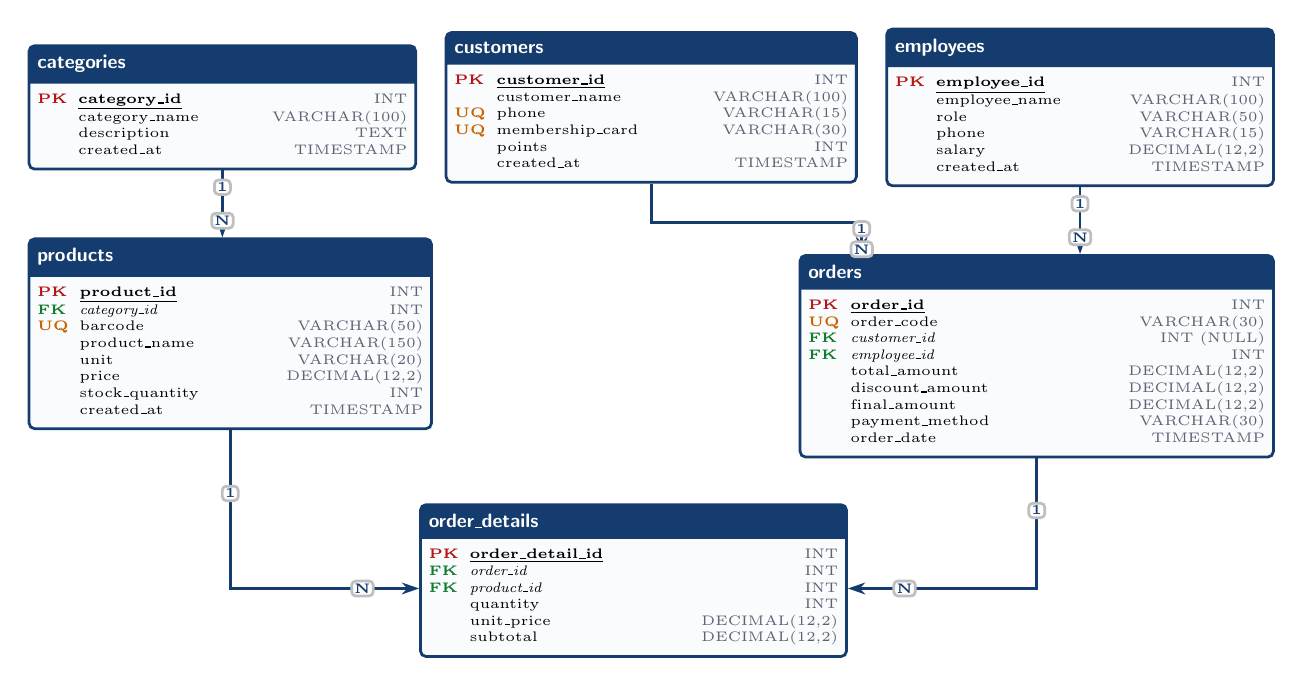
\begin{tikzpicture}[
    entity/.style={
        rectangle split,
        rectangle split parts=2,
        rectangle split part fill={erdblue, erdbg},
        rounded corners=2pt,
        draw=erdblue,
        line width=1pt,
        inner sep=3pt,
        font=\tiny,
        text width=#1,
        align=left
    },
    rel/.style={
        -{Stealth[length=2.2mm, width=1.5mm]},
        line width=1pt,
        color=erdblue
    },
    card/.style={
        font=\bfseries\fontsize{5pt}{6pt}\selectfont,
        fill=white,
        inner sep=1pt,
        rounded corners=1.5pt,
        draw=gray!50
    }
]

% ================= LAYER 1: MASTER DATA =================
\node (cat) [entity=4.7cm] {
    \centering\textbf{\textsf{\textcolor{white}{\scriptsize categories}}}
    \nodepart{two}
    \begin{tabular*}{\linewidth}{@{}l@{\hspace{4pt}}l@{\extracolsep{\fill}}r@{}}
    \textbf{\textcolor{pkcolor}{PK}} & \underline{\textbf{category\_id}} & \textcolor{typecolor}{INT} \\
    & category\_name & \textcolor{typecolor}{VARCHAR(100)} \\
    & description & \textcolor{typecolor}{TEXT} \\
    & created\_at & \textcolor{typecolor}{TIMESTAMP} \\
    \end{tabular*}
};

\node (cust) [entity=5.0cm, right=0.35cm of cat] {
    \centering\textbf{\textsf{\textcolor{white}{\scriptsize customers}}}
    \nodepart{two}
    \begin{tabular*}{\linewidth}{@{}l@{\hspace{4pt}}l@{\extracolsep{\fill}}r@{}}
    \textbf{\textcolor{pkcolor}{PK}} & \underline{\textbf{customer\_id}} & \textcolor{typecolor}{INT} \\
    & customer\_name & \textcolor{typecolor}{VARCHAR(100)} \\
    \textbf{\textcolor{uqcolor}{UQ}} & phone & \textcolor{typecolor}{VARCHAR(15)} \\
    \textbf{\textcolor{uqcolor}{UQ}} & membership\_card & \textcolor{typecolor}{VARCHAR(30)} \\
    & points & \textcolor{typecolor}{INT} \\
    & created\_at & \textcolor{typecolor}{TIMESTAMP} \\
    \end{tabular*}
};

\node (emp) [entity=4.7cm, right=0.35cm of cust] {
    \centering\textbf{\textsf{\textcolor{white}{\scriptsize employees}}}
    \nodepart{two}
    \begin{tabular*}{\linewidth}{@{}l@{\hspace{4pt}}l@{\extracolsep{\fill}}r@{}}
    \textbf{\textcolor{pkcolor}{PK}} & \underline{\textbf{employee\_id}} & \textcolor{typecolor}{INT} \\
    & employee\_name & \textcolor{typecolor}{VARCHAR(100)} \\
    & role & \textcolor{typecolor}{VARCHAR(50)} \\
    & phone & \textcolor{typecolor}{VARCHAR(15)} \\
    & salary & \textcolor{typecolor}{DECIMAL(12,2)} \\
    & created\_at & \textcolor{typecolor}{TIMESTAMP} \\
    \end{tabular*}
};

% ================= LAYER 2: TRANSACTION CORE =================
\node (prod) [entity=4.9cm, below=0.85cm of cat.south west, anchor=north west] {
    \centering\textbf{\textsf{\textcolor{white}{\scriptsize products}}}
    \nodepart{two}
    \begin{tabular*}{\linewidth}{@{}l@{\hspace{4pt}}l@{\extracolsep{\fill}}r@{}}
    \textbf{\textcolor{pkcolor}{PK}} & \underline{\textbf{product\_id}} & \textcolor{typecolor}{INT} \\
    \textbf{\textcolor{fkcolor}{FK}} & \textit{category\_id} & \textcolor{typecolor}{INT} \\
    \textbf{\textcolor{uqcolor}{UQ}} & barcode & \textcolor{typecolor}{VARCHAR(50)} \\
    & product\_name & \textcolor{typecolor}{VARCHAR(150)} \\
    & unit & \textcolor{typecolor}{VARCHAR(20)} \\
    & price & \textcolor{typecolor}{DECIMAL(12,2)} \\
    & stock\_quantity & \textcolor{typecolor}{INT} \\
    & created\_at & \textcolor{typecolor}{TIMESTAMP} \\
    \end{tabular*}
};

\node (orders) [entity=5.8cm, below=0.85cm of emp.south east, anchor=north east] {
    \centering\textbf{\textsf{\textcolor{white}{\scriptsize orders}}}
    \nodepart{two}
    \begin{tabular*}{\linewidth}{@{}l@{\hspace{4pt}}l@{\extracolsep{\fill}}r@{}}
    \textbf{\textcolor{pkcolor}{PK}} & \underline{\textbf{order\_id}} & \textcolor{typecolor}{INT} \\
    \textbf{\textcolor{uqcolor}{UQ}} & order\_code & \textcolor{typecolor}{VARCHAR(30)} \\
    \textbf{\textcolor{fkcolor}{FK}} & \textit{customer\_id} & \textcolor{typecolor}{INT (NULL)} \\
    \textbf{\textcolor{fkcolor}{FK}} & \textit{employee\_id} & \textcolor{typecolor}{INT} \\
    & total\_amount & \textcolor{typecolor}{DECIMAL(12,2)} \\
    & discount\_amount & \textcolor{typecolor}{DECIMAL(12,2)} \\
    & final\_amount & \textcolor{typecolor}{DECIMAL(12,2)} \\
    & payment\_method & \textcolor{typecolor}{VARCHAR(30)} \\
    & order\_date & \textcolor{typecolor}{TIMESTAMP} \\
    \end{tabular*}
};

% ================= LAYER 3: JUNCTION DETAILS =================
\path (prod.south) -- (orders.south) coordinate[midway] (layer3_mid);
\node (odetails) [entity=5.2cm, below=0.75cm of layer3_mid, anchor=north] {
    \centering\textbf{\textsf{\textcolor{white}{\scriptsize order\_details}}}
    \nodepart{two}
    \begin{tabular*}{\linewidth}{@{}l@{\hspace{4pt}}l@{\extracolsep{\fill}}r@{}}
    \textbf{\textcolor{pkcolor}{PK}} & \underline{\textbf{order\_detail\_id}} & \textcolor{typecolor}{INT} \\
    \textbf{\textcolor{fkcolor}{FK}} & \textit{order\_id} & \textcolor{typecolor}{INT} \\
    \textbf{\textcolor{fkcolor}{FK}} & \textit{product\_id} & \textcolor{typecolor}{INT} \\
    & quantity & \textcolor{typecolor}{INT} \\
    & unit\_price & \textcolor{typecolor}{DECIMAL(12,2)} \\
    & subtotal & \textcolor{typecolor}{DECIMAL(12,2)} \\
    \end{tabular*}
};

% ================= RELATIONSHIPS =================
% 1. categories (1) -> products (N)
\draw [rel] (cat.south) -- (cat.south |- prod.north)
    node [card, pos=0.25] {1}
    node [card, pos=0.75] {N};

% 2. customers (1) -> orders (N)
\draw [rel] (cust.south) |- ($(orders.north west)+(0.8,0.4)$) -- ($(orders.north west)+(0.8,0)$)
    node [card, pos=0.2] {1}
    node [card, pos=0.85] {N};

% 3. employees (1) -> orders (N)
\draw [rel] (emp.south) -- (emp.south |- orders.north)
    node [card, pos=0.25] {1}
    node [card, pos=0.75] {N};

% 4. products (1) -> order_details (N)
\draw [rel] (prod.south) |- ($(odetails.west)+(0,-0.1)$)
    node [card, pos=0.2] {1}
    node [card, pos=0.85] {N};

% 5. orders (1) -> order_details (N)
\draw [rel] (orders.south) |- ($(odetails.east)+(0,-0.1)$)
    node [card, pos=0.2] {1}
    node [card, pos=0.85] {N};

\end{tikzpicture}
\caption{Sơ đồ Thực thể Liên kết (ERD) Hệ thống CSDL Bán hàng Siêu thị}
\label{fig:erd_supermarket}
\end{figure}

\section{Cấu trúc Chi tiết và Từ điển Dữ liệu}
Từ điển dữ liệu (Data Dictionary) định nghĩa toàn diện tên trường, kiểu dữ liệu, các ràng buộc toàn vẹn và ý nghĩa nghiệp vụ cụ thể cho cả 6 bảng thực thể trong hệ thống.

\subsection{Bảng Danh mục Ngành hàng (\texttt{categories})}
Bảng \texttt{categories} lưu trữ hệ thống phân loại ngành hàng trong siêu thị (như Thực phẩm tươi sống, Hóa mỹ phẩm, Gia vị, Đồ uống), giúp tổ chức cây sản phẩm khoa học.

\begin{table}[H]
\centering
\footnotesize
\caption{Cấu trúc chi tiết bảng \texttt{categories}}
\label{tab:dict_categories}
\vspace{0.2cm}
\begin{tabularx}{\textwidth}{L{3.3cm} L{2.9cm} L{3.6cm} Y}
\toprule
\textbf{Tên cột} & \textbf{Kiểu dữ liệu} & \textbf{Ràng buộc} & \textbf{Ý nghĩa nghiệp vụ} \\
\midrule
\texttt{category\_id} & INT & PK, AUTO\_INCREMENT & Mã định danh duy nhất của ngành hàng \\
\texttt{category\_name} & VARCHAR(100) & NOT NULL & Tên phân loại ngành hàng siêu thị \\
\texttt{description} & TEXT & NULL & Diễn giải mô tả chi tiết ngành hàng \\
\texttt{created\_at} & TIMESTAMP & DEFAULT CURRENT\_TIMESTAMP & Thời điểm khởi tạo bản ghi ngành hàng \\
\bottomrule
\end{tabularx}
\end{table}

\subsection{Bảng Sản phẩm và Hàng hóa (\texttt{products})}
Bảng \texttt{products} là thực thể trung tâm quản lý danh mục hàng hóa lưu thông tại siêu thị, bao gồm mã vạch tra cứu, đơn vị tính, đơn giá niêm yết và số lượng hàng tồn kho.

\begin{table}[H]
\centering
\footnotesize
\caption{Cấu trúc chi tiết bảng \texttt{products}}
\label{tab:dict_products}
\vspace{0.2cm}
\begin{tabularx}{\textwidth}{L{3.3cm} L{2.9cm} L{3.6cm} Y}
\toprule
\textbf{Tên cột} & \textbf{Kiểu dữ liệu} & \textbf{Ràng buộc} & \textbf{Ý nghĩa nghiệp vụ} \\
\midrule
\texttt{product\_id} & INT & PK, AUTO\_INCREMENT & Mã định danh nội bộ duy nhất của sản phẩm \\
\texttt{barcode} & VARCHAR(50) & UNIQUE, NOT NULL & Mã vạch quốc tế phục vụ quét POS nhanh \\
\texttt{product\_name} & VARCHAR(150) & NOT NULL & Tên hàng hóa hiển thị trên bao bì và hóa đơn \\
\texttt{category\_id} & INT & FK $\to$ \texttt{categories}, NOT NULL & Ngành hàng trực thuộc của sản phẩm \\
\texttt{unit} & VARCHAR(20) & NOT NULL, DEFAULT 'Cái' & Đơn vị tính (Cái, Hộp, Chai, Lon, Gói, Kg) \\
\texttt{price} & DECIMAL(12,2) & NOT NULL & Đơn giá bán lẻ niêm yết hiện hành \\
\texttt{stock\_quantity} & INT & NOT NULL, DEFAULT 0 & Số lượng sản phẩm khả dụng trong kho \\
\texttt{created\_at} & TIMESTAMP & DEFAULT CURRENT\_TIMESTAMP & Thời điểm tiếp nhận mặt hàng vào hệ thống \\
\bottomrule
\end{tabularx}
\end{table}

\subsection{Bảng Khách hàng và Thẻ Thành viên (\texttt{customers})}
Bảng \texttt{customers} quản lý dữ liệu người tiêu dùng thân thiết, phục vụ các chính sách tích lũy điểm thưởng và chăm sóc khách hàng.

\begin{table}[H]
\centering
\footnotesize
\caption{Cấu trúc chi tiết bảng \texttt{customers}}
\label{tab:dict_customers}
\vspace{0.2cm}
\begin{tabularx}{\textwidth}{L{3.3cm} L{2.9cm} L{3.6cm} Y}
\toprule
\textbf{Tên cột} & \textbf{Kiểu dữ liệu} & \textbf{Ràng buộc} & \textbf{Ý nghĩa nghiệp vụ} \\
\midrule
\texttt{customer\_id} & INT & PK, AUTO\_INCREMENT & Mã định danh khách hàng trong hệ thống \\
\texttt{customer\_name} & VARCHAR(100) & NOT NULL & Họ và tên đầy đủ của khách hàng \\
\texttt{phone} & VARCHAR(15) & UNIQUE, NULL & Số điện thoại dùng để tra cứu tại quầy thu ngân \\
\texttt{membership\_card} & VARCHAR(30) & UNIQUE, NULL & Mã thẻ hội viên thân thiết (VIP, Diamond) \\
\texttt{points} & INT & DEFAULT 0 & Điểm thưởng tích lũy qua các đơn hàng \\
\texttt{created\_at} & TIMESTAMP & DEFAULT CURRENT\_TIMESTAMP & Thời điểm đăng ký hồ sơ hội viên \\
\bottomrule
\end{tabularx}
\end{table}

\newpage
\subsection{Bảng Nhân viên và Thu ngân (\texttt{employees})}
Bảng \texttt{employees} ghi nhận đội ngũ nhân sự siêu thị, xác định trách nhiệm của từng nhân viên thu ngân đối với các giao dịch tài chính phát sinh.

\begin{table}[H]
\centering
\footnotesize
\caption{Cấu trúc chi tiết bảng \texttt{employees}}
\label{tab:dict_employees}
\vspace{0.2cm}
\begin{tabularx}{\textwidth}{L{3.3cm} L{2.9cm} L{3.6cm} Y}
\toprule
\textbf{Tên cột} & \textbf{Kiểu dữ liệu} & \textbf{Ràng buộc} & \textbf{Ý nghĩa nghiệp vụ} \\
\midrule
\texttt{employee\_id} & INT & PK, AUTO\_INCREMENT & Mã định danh nhân sự duy nhất \\
\texttt{employee\_name} & VARCHAR(100) & NOT NULL & Họ và tên nhân viên siêu thị \\
\texttt{role} & VARCHAR(50) & DEFAULT 'Thu ngân' & Chức danh công việc (Thu ngân, Quản lý kho) \\
\texttt{phone} & VARCHAR(15) & NULL & Số điện thoại liên hệ nội bộ \\
\texttt{salary} & DECIMAL(12,2) & DEFAULT 0 & Mức lương cơ sở phục vụ quản lý nhân sự \\
\texttt{created\_at} & TIMESTAMP & DEFAULT CURRENT\_TIMESTAMP & Ngày ký hợp đồng làm việc tại siêu thị \\
\bottomrule
\end{tabularx}
\end{table}

\subsection{Bảng Hóa đơn Bán lẻ (\texttt{orders})}
Bảng \texttt{orders} lưu vết tổng hợp của từng đơn giao dịch bán hàng tại quầy thu ngân, quản lý tổng tiền, chiết khấu, phương thức thanh toán và thời điểm xuất phiếu.

\begin{table}[H]
\centering
\footnotesize
\caption{Cấu trúc chi tiết bảng \texttt{orders}}
\label{tab:dict_orders}
\vspace{0.2cm}
\begin{tabularx}{\textwidth}{L{3.3cm} L{2.9cm} L{3.6cm} Y}
\toprule
\textbf{Tên cột} & \textbf{Kiểu dữ liệu} & \textbf{Ràng buộc} & \textbf{Ý nghĩa nghiệp vụ} \\
\midrule
\texttt{order\_id} & INT & PK, AUTO\_INCREMENT & Mã định danh giao dịch hóa đơn \\
\texttt{order\_code} & VARCHAR(30) & UNIQUE, NOT NULL & Mã biên lai bán lẻ in cho khách hàng \\
\texttt{customer\_id} & INT & FK $\to$ \texttt{customers}, NULL & Mã khách mua (NULL nếu là khách vãng lai) \\
\texttt{employee\_id} & INT & FK $\to$ \texttt{employees}, NOT NULL & Nhân viên thu ngân xử lý và in hóa đơn \\
\texttt{total\_amount} & DECIMAL(12,2) & NOT NULL, DEFAULT 0 & Tổng giá trị nguyên giá trước chiết khấu \\
\texttt{discount\_amount} & DECIMAL(12,2) & DEFAULT 0 & Số tiền giảm trừ ưu đãi hoặc điểm hội viên \\
\texttt{final\_amount} & DECIMAL(12,2) & NOT NULL, DEFAULT 0 & Tổng số tiền thực tế khách hàng phải trả \\
\texttt{payment\_method} & VARCHAR(30) & DEFAULT 'Tiền mặt' & Hình thức thanh toán (Tiền mặt, Thẻ POS,...) \\
\texttt{order\_date} & TIMESTAMP & DEFAULT CURRENT\_TIMESTAMP & Thời điểm thực hiện thanh toán giao dịch \\
\bottomrule
\end{tabularx}
\end{table}

\newpage
\subsection{Bảng Chi tiết Hóa đơn Bán lẻ (\texttt{order\_details})}
Bảng \texttt{order\_details} lưu trữ từng mặt hàng thành phần trong mỗi hóa đơn bán lẻ, đảm bảo nguyên tắc kế toán về đơn giá và tính thành tiền.

\begin{table}[H]
\centering
\footnotesize
\caption{Cấu trúc chi tiết bảng \texttt{order\_details}}
\label{tab:dict_order_details}
\vspace{0.2cm}
\begin{tabularx}{\textwidth}{L{3.3cm} L{2.9cm} L{3.6cm} Y}
\toprule
\textbf{Tên cột} & \textbf{Kiểu dữ liệu} & \textbf{Ràng buộc} & \textbf{Ý nghĩa nghiệp vụ} \\
\midrule
\texttt{order\_detail\_id} & INT & PK, AUTO\_INCREMENT & Mã định danh dòng chi tiết hóa đơn \\
\texttt{order\_id} & INT & FK $\to$ \texttt{orders}, NOT NULL & Mã hóa đơn chứa mặt hàng \\
\texttt{product\_id} & INT & FK $\to$ \texttt{products}, NOT NULL & Mã sản phẩm được khách chọn mua \\
\texttt{quantity} & INT & NOT NULL & Số lượng sản phẩm khách mua trong đơn \\
\texttt{unit\_price} & DECIMAL(12,2) & NOT NULL & Đơn giá bán thực tế tại thời điểm lập hóa đơn \\
\texttt{subtotal} & DECIMAL(12,2) & NOT NULL & Thành tiền mặt hàng ($= \text{quantity} \times \text{unit\_price}$) \\
\bottomrule
\end{tabularx}
\end{table}

\section{Các Quyết định Thiết kế Nghiệp vụ và Tối ưu Hóa Cụm Phân Tán}
Thiết kế CSDL \texttt{supermarket\_db} không chỉ đáp ứng bài toán lưu trữ tĩnh mà còn giải quyết hiệu quả các yêu cầu đặc thù của nghiệp vụ siêu thị và môi trường cụm nhân bản MySQL:

\subsection{Tối ưu Hóa Tra cứu Mã Vạch Điểm Bán POS}
\noindent\textbf{Vấn đề nghiệp vụ:} Trong môi trường bán lẻ tại quầy POS, thu ngân liên tục dùng máy quét mã vạch để đọc các mã định danh sản phẩm. Nếu hệ thống phải thực hiện quét toàn bảng trên hàng chục nghìn sản phẩm, thời gian phản hồi sẽ tăng đột biến, gây nghẽn quầy thu ngân trong giờ cao điểm.

\vspace{0.2cm}
\noindent\textbf{Giải pháp thiết kế:} Thuộc tính \texttt{barcode} trong bảng \texttt{products} được thiết lập ràng buộc duy nhất \texttt{UNIQUE NOT NULL}. Trong công nghệ lưu trữ InnoDB, định nghĩa này tự động khởi tạo một chỉ mục B+Tree duy nhất (Unique B-Tree Index). Độ phức tạp của thao tác tra cứu sản phẩm theo mã vạch đạt mức $O(\log N) \approx O(1)$ vì cấu trúc B+Tree chỉ gồm 2--3 tầng chỉ mục. Nhờ đó, thời gian phản hồi quét mã vạch luôn ổn định ở mức $< 1\text{ms}$ bất kể dung lượng dữ liệu tăng trưởng.

\subsection{Bảo Toàn Lịch Sử Đơn Giá Giao Dịch}
\noindent\textbf{Vấn đề nghiệp vụ:} Giá bán lẻ của hàng hóa trong bảng \texttt{products} thường xuyên biến động theo thời gian do chính sách điều chỉnh giá, lạm phát hoặc các đợt khuyến mãi. Nếu bảng \texttt{order\_details} chỉ tham chiếu động đến \texttt{products.price} mà không lưu giá tĩnh, khi sản phẩm thay đổi giá trong tương lai, tổng tiền của toàn bộ hóa đơn lịch sử trong quá khứ sẽ bị tính toán sai lệch, gây vi phạm nghiêm trọng quy chuẩn kiểm toán tài chính.

\vspace{0.2cm}
\noindent\textbf{Giải pháp thiết kế:} Bảng \texttt{order\_details} được chủ động bổ sung trường \texttt{unit\_price DECIMAL(12,2)}. Khi giao dịch phát sinh, đơn giá tại đúng thời điểm đó được chụp lại và ghi cố định vào dòng chi tiết hóa đơn. Thành tiền \texttt{subtotal} được tính toán dựa trên đơn giá lịch sử này, bảo đảm tính toàn vẹn của số liệu kế toán qua các thời kỳ.

\subsection{Mô Hình Xử Lý Khách Hàng Vãng Lai Linh Hoạt}
\noindent\textbf{Vấn đề nghiệp vụ:} Khách mua hàng tại siêu thị gồm hai nhóm đối tượng: khách hàng thân thiết có thẻ thành viên và khách hàng vãng lai mua sắm ngẫu nhiên. Nếu thiết lập ràng buộc \texttt{customer\_id NOT NULL}, hệ thống sẽ bắt buộc nhân viên phải tạo tài khoản giả lập cho mọi khách vãng lai, gây lãng phí dung lượng lưu trữ và làm chậm tốc độ xuất vé bán hàng. Ngược lại, nếu khách hàng thân thiết hủy tài khoản, các hóa đơn mua sắm trong quá khứ của họ không được phép biến mất khỏi hệ thống báo cáo doanh thu.

\vspace{0.2cm}
\noindent\textbf{Giải pháp thiết kế:} Trường \texttt{customer\_id} trong bảng \texttt{orders} được phép nhận giá trị \texttt{NULL} (\texttt{INT NULL}). Đồng thời, quy tắc toàn vẹn khóa ngoại được thiết lập:
\begin{lstlisting}[language=SQL]
CONSTRAINT fk_orders_customers FOREIGN KEY (customer_id) 
REFERENCES customers(customer_id) ON DELETE SET NULL ON UPDATE CASCADE
\end{lstlisting}
Khi khách vãng lai mua hàng, hệ thống ghi nhận \texttt{customer\_id = NULL}. Khi một hồ sơ hội viên bị xóa, các hóa đơn liên quan vẫn được lưu giữ nguyên vẹn với trường \texttt{customer\_id} tự động chuyển sang \texttt{NULL}, bảo toàn dữ liệu báo cáo doanh thu tổng của siêu thị.

\subsection{Ràng Buộc Toàn Vẹn Bảo Vệ Dữ Liệu Kế Toán}
\noindent\textbf{Vấn đề nghiệp vụ:} Thao tác xóa nhầm danh mục hàng hóa, nhân viên bán hàng hoặc thông tin mặt hàng đang có giao dịch phát sinh sẽ tạo ra các bản ghi mồ côi, làm sai lệch toàn bộ báo cáo doanh số và quy trình đối soát công nợ.

\vspace{0.2cm}
\noindent\textbf{Giải pháp thiết kế:} Hệ thống áp dụng quy tắc khóa nghiêm ngặt \texttt{ON DELETE RESTRICT} trên các mối quan hệ trọng yếu:
\begin{itemize}
    \item \texttt{fk\_products\_categories}: Chặn việc xóa danh mục nếu ngành hàng đó vẫn còn chứa sản phẩm liên kết.
    \item \texttt{fk\_orders\_employees}: Chặn việc xóa hồ sơ nhân viên nếu người đó đã từng thực hiện xuất bất kỳ hóa đơn nào.
    \item \texttt{fk\_order\_details\_products}: Ngăn chặn việc xóa dữ liệu sản phẩm nếu mặt hàng đã từng xuất hiện trong lịch sử mua hàng của khách.
\end{itemize}
Nhờ đó, tính toàn vẹn tham chiếu của cơ sở dữ liệu được MySQL kiểm soát ngay ở tầng lưu trữ, hạn chế đáng kể nguy cơ thao tác nhầm của người vận hành.

\subsection{Thiết Kế Tương Thích Với Cụm Nhân Bản MySQL (GTID và InnoDB)}
\noindent\textbf{Đặc thù phân tán:} Cụm cơ sở dữ liệu vận hành theo mô hình Master-Slave với cơ chế định dạng bản ghi nhị phân kết hợp định danh giao dịch toàn cục \textbf{GTID}. Trong kiến trúc này, việc thiết kế lược đồ bảng đóng vai trò quyết định đến hiệu năng sao chép:
\begin{enumerate}
    \item \textbf{Sử dụng thống nhất Engine InnoDB:} Tất cả 6 bảng đều sử dụng động cơ \texttt{InnoDB} với bảng mã \texttt{utf8mb4\_unicode\_ci}. InnoDB hỗ trợ cơ chế khóa ở cấp độ dòng và tính năng tự khôi phục sau sự cố, tương thích tốt với tham số an toàn giao dịch \texttt{innodb\_flush\_log\_at\_trx\_commit = 1}.
    \item \textbf{Bắt buộc khóa chính số nguyên \texttt{AUTO\_INCREMENT PRIMARY KEY}:} Mọi bảng đều sở hữu một khóa chính duy nhất kiểu số nguyên tự tăng. Khi thực hiện sao chép định dạng \texttt{ROW}, các node Slave sử dụng khóa chính để tìm nạp trực tiếp dòng dữ liệu cần sửa đổi/xóa qua chỉ mục Clustered Index ($O(1)$). Nếu thiếu khóa chính, Slave buộc phải quét toàn bộ bảng cho mỗi bản ghi trong Binary Log, dẫn đến hiện tượng trễ nhân bản nghiêm trọng và làm nghẽn cụm.
    \item \textbf{Định danh giao dịch duy nhất cho hóa đơn (\texttt{order\_code UNIQUE}):} Ngăn chặn nguy cơ trùng lặp mã hóa đơn khi hệ thống mở rộng quy mô phục vụ nhiều cổng thanh toán đồng thời.
\end{enumerate}

% ------------------------------------------------------------------------------
% CHƯƠNG 3
% ------------------------------------------------------------------------------
\chapter{Quy Trình Cài Đặt Và Cấu Hình Cụm}

Quy trình triển khai thực tế cụm cơ sở dữ liệu phân tán 1 Master -- 2 Slave cho hệ thống quản lý bán hàng siêu thị được tự động hóa theo 4 giai đoạn tuần tự: (1) Khởi tạo hạ tầng container và mạng nội bộ bằng Docker Compose; (2) Tinh chỉnh tham số engine MySQL tách biệt giữa Master và Slave; (3) Thiết lập kết nối nhân bản tự động theo chuẩn GTID; và (4) Nạp dữ liệu nghiệp vụ ban đầu kết hợp nghiệm thu trạng thái đồng bộ toàn cụm.

Toàn bộ mã nguồn cấu hình, lược đồ SQL và bộ kịch bản kiểm thử đã được nhóm công khai tại kho lưu trữ GitHub: \url{https://github.com/Sonsiunhan/DBMS_Cluster} (đồng thời mã nguồn SQL khởi tạo bảng cũng được đính kèm đầy đủ tại Phụ lục~\ref{chap:appendix_sql} để có thể dựng thủ công trực tiếp từ báo cáo). Để tái lập nhanh toàn bộ cụm 2,62 triệu bản ghi và chạy kiểm thử, thực hiện các lệnh sau:

\begin{lstlisting}[language=bash, caption={Lệnh tải mã nguồn và khởi tạo tự động toàn bộ cụm từ kho lưu trữ GitHub}]
git clone https://github.com/Sonsiunhan/DBMS_Cluster.git
cd DBMS_Cluster && docker compose up -d
bash ./scripts/04_seed_million_records.sh
bash ./scripts/02_verify_replication.sh
\end{lstlisting}

\section{Triển khai Hạ tầng với Docker Compose}
Tệp cấu hình \texttt{docker-compose.yml} tại thư mục gốc định nghĩa tập trung toàn bộ cụm 3 máy chủ MySQL 8.0, đảm bảo tính đồng nhất về phiên bản hệ quản trị, không gian mạng và ổ đĩa lưu trữ bền vững mỗi khi khởi tạo môi trường:

\begin{lstlisting}[caption={Cấu hình triển khai cụm 3 node trong tệp docker-compose.yml}]
services:
  mysql-master:
    image: mysql:8.0
    container_name: mysql-master
    restart: always
    environment:
      MYSQL_ROOT_PASSWORD: rootpassword
      MYSQL_DATABASE: supermarket_db
    ports:
      - "3306:3306"
    volumes:
      - ./config/master/my.cnf:/etc/mysql/conf.d/my.cnf:ro
      - master_data:/var/lib/mysql
    networks:
      - dbms-net

  mysql-slave-1:
    image: mysql:8.0
    container_name: mysql-slave-1
    restart: always
    environment:
      MYSQL_ROOT_PASSWORD: rootpassword
    ports:
      - "3307:3306"
    volumes:
      - ./config/slave1/my.cnf:/etc/mysql/conf.d/my.cnf:ro
      - slave1_data:/var/lib/mysql
    depends_on:
      - mysql-master
    networks:
      - dbms-net

  mysql-slave-2:
    image: mysql:8.0
    container_name: mysql-slave-2
    restart: always
    environment:
      MYSQL_ROOT_PASSWORD: rootpassword
    ports:
      - "3308:3306"
    volumes:
      - ./config/slave2/my.cnf:/etc/mysql/conf.d/my.cnf:ro
      - slave2_data:/var/lib/mysql
    depends_on:
      - mysql-master
    networks:
      - dbms-net

networks:
  dbms-net:
    driver: bridge

volumes:
  master_data:
  slave1_data:
  slave2_data:
\end{lstlisting}

Trong cấu hình triển khai trên, ba nguyên tắc kỹ thuật quan trọng được áp dụng:
\begin{itemize}
    \item \textbf{Gắn kết cấu hình ở chế độ chỉ đọc (\texttt{:ro}):} Mỗi tệp \texttt{my.cnf} riêng biệt của từng trạm được ánh xạ trực tiếp vào đường dẫn \texttt{/etc/mysql/conf.d/my.cnf} bên trong container với cờ \texttt{read-only}, ngăn chặn mọi thao tác ghi đè cấu hình ngoài ý muốn trong quá trình vận hành.
    \item \textbf{Khởi tạo CSDL gốc có kiểm soát:} Biến môi trường \texttt{MYSQL\_DATABASE} trên máy chủ \texttt{mysql-master} được gán giá trị \texttt{supermarket\_db} nhằm tự động khởi tạo không gian tên CSDL ngay lần chạy đầu tiên, sẵn sàng tiếp nhận lược đồ bảng và phân phối sang các trạm phụ thuộc.
    \item \textbf{Kích hoạt cụm dịch vụ nền:} Cụm container được khởi chạy đồng loạt bằng lệnh \texttt{docker compose up -d}. Nhờ chỉ thị \texttt{depends\_on} và \texttt{restart: always}, tiến trình \texttt{mysqld} trên cả 3 node tự động khởi động tuần tự và duy trì trạng thái trực tuyến liên tục.
\end{itemize}

\section{Cấu hình Tham số MySQL trên Master và Slave}
Mặc dù cùng chạy MySQL 8.0, tệp cấu hình \texttt{my.cnf} giữa máy chủ chính và hai bản sao được thiết kế đối xứng nhưng phân tách rõ rệt theo vai trò đọc -- ghi.

\subsection{Cấu hình trên Máy chủ Master}
Tệp \texttt{config/master/my.cnf} định nghĩa máy chủ Master làm điểm tiếp nhận giao dịch ghi duy nhất và là nguồn phát nhật ký sự kiện cho toàn cụm:

\begin{lstlisting}[caption={Cấu hình tham số my.cnf trên máy chủ Master}]
[mysqld]
server-id = 1
log-bin = mysql-bin
binlog_format = ROW
binlog-do-db = supermarket_db
gtid_mode = ON
enforce_gtid_consistency = ON
sync_binlog = 1
innodb_flush_log_at_trx_commit = 1
binlog_expire_logs_seconds = 604800
max_binlog_size = 100M
\end{lstlisting}

Trên Master, tham số \texttt{binlog\_format = ROW} bắt buộc hệ quản trị ghi nhận sự thay đổi dữ liệu ở mức từng dòng bản ghi thực tế thay vì câu lệnh SQL thuần túy, ngăn ngừa hiệu quả nguy cơ sai lệch dữ liệu khi sử dụng các hàm phi tất định như \texttt{NOW()} hay \texttt{UUID()}. Đồng thời, \texttt{binlog-do-db = supermarket\_db} giúp cô lập luồng nhân bản chỉ tập trung vào CSDL nghiệp vụ siêu thị, bỏ qua các bảng hệ thống nội bộ.

\subsection{Cấu hình trên hai Máy chủ Slave}
Hai tệp \texttt{config/slave1/my.cnf} và \texttt{config/slave2/my.cnf} được cấu hình đồng nhất về cơ chế bảo vệ và nhân bản, chỉ khác biệt ở mã định danh nút mạng (\texttt{server-id = 2} đối với Slave 1 và \texttt{server-id = 3} đối với Slave 2):

\begin{lstlisting}[caption={Cấu hình tham số my.cnf trên máy chủ Slave 1 (Slave 2 đặt server-id = 3)}]
[mysqld]
server-id = 2
relay-log = mysql-relay-bin
log-bin = mysql-bin
read_only = 1
super_read_only = 1
replicate-do-db = supermarket_db
gtid_mode = ON
enforce_gtid_consistency = ON
relay_log_recovery = ON
log_replica_updates = ON
sync_binlog = 1
innodb_flush_log_at_trx_commit = 1
binlog_expire_logs_seconds = 604800
max_binlog_size = 100M
\end{lstlisting}

So với Master, tệp cấu hình của Slave bổ sung ba nhóm tham số chuyên biệt: (1) Khai báo nhật ký trung chuyển \texttt{relay-log} (\texttt{mysql-relay-bin}) và bộ lọc \texttt{replicate-do-db} giới hạn ở CSDL \texttt{supermarket\_db}; (2) Kích hoạt khóa ghi hai lớp \texttt{read\_only = 1} và \texttt{super\_read\_only = 1} để chặn đứng mọi truy vấn chỉnh sửa dữ liệu trực tiếp từ phía ứng dụng hoặc quản trị viên; (3) Bật đồng thời \texttt{log-bin} và \texttt{log\_replica\_updates = ON} để Slave tự ghi lại các sự kiện nhận từ Master vào Binary Log cục bộ của chính nó, đảm bảo khả năng sẵn sàng thăng hạng làm Master mới ngay khi xảy ra thảm họa.

\section{Thiết lập Kết nối Nhân bản Tự động}
Sau khi cả 3 container khởi chạy ổn định, quá trình kết nối luồng nhân bản được tự động hóa hoàn toàn thông qua kịch bản \texttt{scripts/01\_setup\_replication.sh} gồm hai bước cốt lõi:

\textbf{Bước 1 -- Khởi tạo tài khoản nhân bản chuyên dụng trên Master:} Thay vì sử dụng tài khoản quản trị mặc định \texttt{root} tiềm ẩn rủi ro bảo mật, nhóm khởi tạo tài khoản riêng \texttt{repl\_user} chỉ được cấp duy nhất đặc quyền \texttt{REPLICATION SLAVE}. Phương thức xác thực \texttt{mysql\_native\_password} được chỉ định rõ ràng nhằm đảm bảo luồng I/O Thread trên các Slave bắt tay qua kết nối mạng nội bộ Docker không gặp rào cản trao đổi khóa RSA công khai của MySQL 8.0:

\begin{lstlisting}[language=SQL, caption={Khởi tạo và phân quyền tài khoản nhân bản trên Master}]
CREATE USER IF NOT EXISTS 'repl_user'@'%'
  IDENTIFIED WITH mysql_native_password BY 'repl_password';
GRANT REPLICATION SLAVE ON *.* TO 'repl_user'@'%';
FLUSH PRIVILEGES;
\end{lstlisting}

\textbf{Bước 2 -- Kích hoạt đồng bộ tự động theo GTID trên cả 2 Slave:} Trên từng máy \texttt{mysql-slave-1} và \texttt{mysql-slave-2}, luồng nhân bản được trỏ trực tiếp tới định danh DNS nội bộ \texttt{mysql-master} ở cổng \texttt{3306} kèm cờ tự động định vị \texttt{SOURCE\_AUTO\_POSITION = 1}:

\begin{lstlisting}[language=SQL, caption={Thiết lập nguồn nhân bản GTID trên Slave 1 và Slave 2}]
STOP REPLICA;
CHANGE REPLICATION SOURCE TO
  SOURCE_HOST = 'mysql-master',
  SOURCE_USER = 'repl_user',
  SOURCE_PASSWORD = 'repl_password',
  SOURCE_PORT = 3306,
  SOURCE_AUTO_POSITION = 1;
START REPLICA;
\end{lstlisting}

\section{Khởi tạo Dữ liệu Siêu thị và Xác minh Trạng thái Đồng bộ}

\subsection{Nạp Lược đồ và Mở rộng Quy mô Hàng triệu Bản ghi}
Khi kênh nhân bản đã thông suốt, cấu trúc bảng nền tảng và dữ liệu mẫu của siêu thị (chi tiết mã SQL tại Phụ lục~\ref{chap:appendix_sql}) được khởi tạo tập trung tại cổng vào của \texttt{mysql-master} kèm kịch bản sinh tải \texttt{04\_seed\_million\_records.sh}:

\begin{lstlisting}[language=bash, caption={Nạp lược đồ gốc và sinh 2,62 triệu bản ghi trên Master}]
docker exec -i mysql-master mysql -uroot -prootpassword \
  supermarket_db < sql/01_schema.sql
docker exec -i mysql-master mysql -uroot -prootpassword \
  supermarket_db < sql/02_sample_data.sql
./scripts/04_seed_million_records.sh
\end{lstlisting}

Thay vì chèn đơn lẻ từng bản ghi gây nghẽn I/O đĩa dưới cơ chế \texttt{sync\_binlog = 1}, kịch bản \texttt{04\_seed\_million\_records.sh} ứng dụng truy vấn tập hợp đệ quy (\texttt{WITH RECURSIVE}) để chèn theo từng lô từ $50.000$ đến $100.000$ dòng/giao dịch. Binary Log lập tức đóng gói các lô sự kiện kèm mã GTID và nhân bản tự động sang cả hai máy Slave, nâng quy mô mỗi node lên chính xác \textbf{2.620.520 bản ghi}.

\subsection{Nghiệm thu Trạng thái Luồng Nhân bản và Đối soát Bản ghi}
Để xác nhận cụm phân tán vận hành chuẩn xác sau khi nạp khối lượng dữ liệu lớn, nhóm thực hiện kiểm tra chéo thông qua câu lệnh \texttt{SHOW REPLICA STATUS\textbackslash G} kết hợp cùng kịch bản tự động \texttt{02\_verify\_replication.sh} trong thư mục \texttt{scripts/}. Bảng~\ref{tab:verify_replica_status} tổng hợp các chỉ số cốt lõi ghi nhận trên cả hai máy Slave.

\begin{table}[H]
\centering
\footnotesize
\caption{Kết quả kiểm tra các chỉ số trạng thái nhân bản trên Slave 1 và Slave 2}
\label{tab:verify_replica_status}
\vspace{0.15cm}
\begin{tabularx}{\textwidth}{L{4.2cm} L{3.5cm} Y}
\toprule
\textbf{Tham số trạng thái} & \textbf{Giá trị ghi nhận} & \textbf{Ý nghĩa nghiệm thu kỹ thuật} \\
\midrule
\texttt{Source\_Host} & \texttt{mysql-master} & Kết nối đúng tới định danh DNS của máy chủ nguồn trong mạng \texttt{dbms-net}. \\
\texttt{Replica\_IO\_Running} & \texttt{Yes} & Luồng I/O Thread đang kết nối tốt và nhận Binary Log liên tục từ Master. \\
\texttt{Replica\_SQL\_Running} & \texttt{Yes} & Luồng SQL Applier đang đọc Relay Log và thực thi dữ liệu vào InnoDB ổn định. \\
\texttt{Auto\_Position} & \texttt{1} & Cơ chế tự động định vị và bù giao dịch theo tập hợp GTID đã được kích hoạt. \\
\texttt{Seconds\_Behind\_Source} & \texttt{0} & Độ trễ nhân bản bằng 0 giây, luồng nhân bản bất đồng bộ trên Slave đã bắt kịp hoàn toàn với Master. \\
\texttt{Last\_Error} & \textit{(Trống)} & Không phát sinh bất kỳ xung đột khóa ngoại hay lỗi cú pháp nào trên luồng nhân bản. \\
\bottomrule
\end{tabularx}
\end{table}

Cuối cùng, kịch bản \texttt{02\_verify\_replication.sh} thực thi truy vấn \texttt{UNION ALL} đếm số dòng của cả 6 bảng trên ba máy chủ Master, Slave 1 và Slave 2. Kết quả đối soát khớp nhau hoàn toàn ở mốc \textbf{2.620.520 bản ghi/node} (tổng cộng \textbf{7.861.560 bản ghi} trên toàn cụm), xác nhận hệ thống đã sẵn sàng cho giai đoạn thực nghiệm tại Chương 4.

% ------------------------------------------------------------------------------
% CHƯƠNG 4
% ------------------------------------------------------------------------------
\chapter{Kết Quả Thực Nghiệm Chi Tiết}

Nhóm đã xây dựng và kiểm thử \textbf{8 ca thực nghiệm} trên nền cơ sở dữ liệu quy mô \textbf{2.620.520 bản ghi/node}, mô phỏng các tình huống vận hành điển hình, sự cố hạ tầng và áp lực tải cao điểm của chuỗi siêu thị. Toàn bộ 8 ca dưới đây được trình bày thống nhất theo cấu trúc: mục tiêu kiểm thử, kịch bản lệnh thực thi, bảng số liệu đối soát thực tế và phân tích kết quả (ảnh chụp màn hình Terminal đối chứng được tổng hợp tại Phụ lục~\ref{chap:appendix}).

\section{Ca 1: Đồng bộ Dữ liệu Bán hàng Xuôi}
\textbf{Mục tiêu:} Kiểm chứng các thao tác thêm mới giao dịch, cập nhật tồn kho và xóa dữ liệu hợp lệ phát sinh trên \texttt{mysql-master} được nhân bản nhanh chóng và chính xác sang cả hai máy Slave.

Kịch bản \texttt{01\_test\_dml\_replication.sh} thực thi tuần tự cả ba nhóm câu lệnh DML trên máy chủ Master như trình bày tại Listing~\ref{lst:ca1_dml}:

\begin{lstlisting}[language=SQL, label={lst:ca1_dml}, caption={Chuỗi thao tác INSERT, UPDATE và DELETE thực thi trên Master (Ca 1)}]
-- 1. INSERT: Dang ky khach hang moi (ID=100001) va xuat hoa don ban le
INSERT INTO customers (customer_name, phone, membership_card, points)
VALUES ('Ngo Hoang Long', '0988275940', 'VIP27594', 100);
SET @cust_id = LAST_INSERT_ID();
INSERT INTO orders (order_code, customer_id, employee_id,
                    total_amount, discount_amount, final_amount, payment_method)
VALUES ('HD_CA1_1795627594', @cust_id, 1, 125000, 0, 125000, 'Chuyen khoan');
SET @order_id = LAST_INSERT_ID();
INSERT INTO order_details (order_id, product_id, quantity, unit_price, subtotal)
VALUES (@order_id, 1, 1, 52000, 52000), (@order_id, 9, 1, 73000, 73000);
-- 2. UPDATE: Khau tru ton kho hai mat hang vua xuat ban (ID=1 va ID=9)
UPDATE products SET stock_quantity = stock_quantity - 1 WHERE product_id IN (1, 9);
-- 3. DELETE: Tao danh muc khuyen mai ngan han va xoa hop le
INSERT INTO categories (category_name, description) VALUES ('Temp_Promo', 'Short-term');
DELETE FROM categories WHERE category_name = 'Temp_Promo';
\end{lstlisting}

\begin{table}[H]
\centering
\footnotesize
\caption{Kết quả đối chiếu dữ liệu trên cả 3 Node sau chuỗi thao tác DML (Ca 1)}
\label{tab:ca1_results}
\vspace{0.15cm}
\begin{tabularx}{\textwidth}{L{1.9cm} Y L{2.8cm} L{2.8cm} L{2.8cm}}
\toprule
\textbf{Thao tác} & \textbf{Đối tượng kiểm tra} & \textbf{Master} & \textbf{Slave 1} & \textbf{Slave 2} \\
\midrule
\texttt{INSERT} & Hóa đơn \texttt{HD\_CA1\_1795627594} (\texttt{customer\_id = 100001}) & \texttt{125.000,00} & \texttt{125.000,00} & \texttt{125.000,00} \\
\texttt{UPDATE} & Tồn kho SP \texttt{ID=1} (trước: \texttt{120}) & \texttt{119} chai & \texttt{119} chai & \texttt{119} chai \\
\texttt{UPDATE} & Tồn kho SP \texttt{ID=9} (trước: \texttt{40}) & \texttt{39} hộp & \texttt{39} hộp & \texttt{39} hộp \\
\texttt{DELETE} & Danh mục tạm sự kiện ngắn hạn & \texttt{0 rows} (Đã xóa) & \texttt{0 rows} (Đã xóa) & \texttt{0 rows} (Đã xóa) \\
\bottomrule
\end{tabularx}
\end{table}

\noindent \textbf{Nhận xét kết quả:} Dữ liệu trên cả ba node khớp nhau hoàn toàn sau khi thực thi với thời gian lan truyền dưới $10\text{ ms}$, dải \texttt{Executed\_Gtid\_Set} trên Master, Slave 1 và Slave 2 đồng nhất tại mốc \texttt{daedfed3-...:1-6} (xem Hình~\ref{fig:ca1}, Phụ lục~\ref{chap:appendix}).

\section{Ca 2: Bảo vệ Tính Toàn vẹn với Khóa Ghi Độc quyền}
\textbf{Mục tiêu:} Kiểm chứng các trạm Slave từ chối các thao tác ghi trực tiếp từ ứng dụng và quản trị viên bên ngoài nhờ chế độ \texttt{super\_read\_only = 1}, nhưng vẫn miễn trừ cho luồng Replication Applier từ Master.

Kịch bản \texttt{02\_test\_readonly\_protection.sh} gửi trực tiếp ba lệnh ghi trái phép vào hai máy Slave (bằng tài khoản quản trị \texttt{root}), sau đó đối chứng khả năng truy vấn đọc và luồng nhân bản từ Master (Listing~\ref{lst:ca2_readonly}):

\begin{lstlisting}[language=SQL, label={lst:ca2_readonly}, caption={Kiểm thử ghi trái phép trên Slave và đối chứng đồng bộ từ Master (Ca 2)}]
-- 1. Thuc thi truc tiep tren Slave 1 & Slave 2 (tai khoan root) -> Bi chan boi ERROR 1290
INSERT INTO products (barcode, product_name, category_id, unit, price, stock_quantity)
VALUES ('893_FAKE_001', 'Hang khong ro nguon goc', 1, 'Cai', 1000, 100);

UPDATE products SET price = 500 WHERE product_id = 1;
DELETE FROM customers WHERE customer_id = 1;

-- 2. Doi chung: Quay thu ngan truy van doc tren Slave & nhap hang hop le tu Master
SELECT COUNT(*) FROM products;
INSERT INTO products (barcode, product_name, category_id, unit, price, stock_quantity)
VALUES ('893_AUTH_1795627599', 'Nuoc mam Phu Quoc 40 do dam', 5, 'Chai', 65000, 45);
\end{lstlisting}

\begin{table}[H]
\centering
\footnotesize
\caption{Phản hồi của hệ thống trước các thao tác kiểm thử quyền Đọc -- Ghi (Ca 2)}
\label{tab:ca2_results}
\vspace{0.15cm}
\begin{tabularx}{\textwidth}{L{3.5cm} L{2.8cm} Y}
\toprule
\textbf{Thao tác kiểm thử} & \textbf{Node đích} & \textbf{Kết quả phản hồi thực tế từ MySQL Engine} \\
\midrule
\texttt{INSERT} sản phẩm lạ & \texttt{mysql-slave-1} & Chặn đứng: \texttt{ERROR 1290 (HY000): --super-read-only} \\
\texttt{UPDATE} sửa đơn giá & \texttt{mysql-slave-2} & Chặn đứng: \texttt{ERROR 1290 (HY000): --super-read-only} \\
\texttt{DELETE} xóa khách hàng & \texttt{mysql-slave-1} & Chặn đứng: \texttt{ERROR 1290 (HY000): --super-read-only} \\
\texttt{SELECT COUNT(*)} kho & Slave 1 \& Slave 2 & Thành công bình thường: trả về chính xác \texttt{20.000} sản phẩm \\
\texttt{INSERT} từ Master & \texttt{mysql-master} & Thành công; cả 2 Slave tự động nhận \textit{Nước mắm Phú Quốc 40 độ đạm} \\
\bottomrule
\end{tabularx}
\end{table}

\noindent \textbf{Nhận xét kết quả:} Cơ chế khóa ghi hai lớp bảo vệ chặt chẽ dữ liệu tại các trạm bản sao khỏi nguy cơ sai lệch cục bộ (Split-Brain), đồng thời duy trì thông suốt cả luồng đọc POS lẫn luồng nhân bản ngầm từ Master (xem ảnh chụp Terminal tại Hình~\ref{fig:ca2}, Phụ lục~\ref{chap:appendix}).

\section{Ca 3: Gián đoạn Mạng và Tự động Bù Dữ liệu qua GTID}
\textbf{Mục tiêu:} Đánh giá khả năng chịu lỗi (Fault Tolerance) khi một máy Slave bị mất kết nối mạng tạm thời trong lúc siêu thị vẫn liên tục phát sinh giao dịch mới trên Master.

Kịch bản \texttt{03\_test\_fault\_tolerance.sh} chủ động ngắt luồng nhân bản trên Slave 1, ghi nhận hai giao dịch mới trên Master trong thời gian cô lập, sau đó nối lại mạng để kiểm tra cơ chế tự bù giao dịch qua GTID (Listing~\ref{lst:ca3_fault}):

\begin{lstlisting}[language=SQL, label={lst:ca3_fault}, caption={Mô phỏng ngắt kết nối Slave 1, ghi mới trên Master và khôi phục tự động (Ca 3)}]
-- Buoc 1 (Tren Slave 1): Ngat luong nhan ban mo phong su co dut cap mang
STOP REPLICA;

-- Buoc 2 (Tren Master): Sieu thi tiep tuc xuat hoa don va nhap kho khi Slave 1 offline
INSERT INTO orders (order_code, customer_id, employee_id,
                    total_amount, final_amount, payment_method)
VALUES ('HD_OFFLINE_1795627602', 2, 2, 203000, 203000, 'Tien mat');

INSERT INTO products (barcode, product_name, category_id, unit, price, stock_quantity)
VALUES ('893_OFF_1795627602', 'Banh quy bo Danisa (7602g)', 3, 'Hop', 125000, 30);

-- Buoc 3 (Tren Slave 1): Khoi phuc ket noi mang -> GTID tu dong doi chieu va keo bu
START REPLICA;
\end{lstlisting}

\begin{table}[H]
\centering
\footnotesize
\caption{Diễn biến trạng thái luồng và tập hợp GTID trên 3 Node qua các giai đoạn sự cố (Ca 3)}
\label{tab:ca3_results}
\vspace{0.15cm}
\begin{tabularx}{\textwidth}{L{3.7cm} L{2.9cm} L{4.2cm} Y}
\toprule
\textbf{Giai đoạn kiểm thử} & \textbf{Master} & \textbf{Slave 1 (Sự cố mạng)} & \textbf{Slave 2 (Bình thường)} \\
\midrule
1. Ngắt mạng Slave 1 & \texttt{...:1-23} & \texttt{...:1-23} (\texttt{IO/SQL: No}) & \texttt{...:1-23} (\texttt{IO/SQL: Yes}) \\
2. Master ghi 2 giao dịch & \texttt{...:1-25} & \texttt{...:1-23} (Thiếu 2 giao dịch) & \texttt{...:1-25} (Nhận tức thời) \\
3. Khôi phục \texttt{START REPLICA} & \texttt{...:1-25} & \texttt{...:1-25} (Tự bù đủ 100\%) & \texttt{...:1-25} (Đồng nhất) \\
\bottomrule
\end{tabularx}
\end{table}

\noindent \textbf{Nhận xét kết quả:} Ngay khi kết nối mạng khôi phục, cờ \texttt{SOURCE\_AUTO\_POSITION = 1} thực hiện phép hiệu tập hợp toán học giữa Master (\texttt{1-25}) và Slave 1 (\texttt{1-23}), tự động truyền bù chính xác 2 giao dịch thiếu (\texttt{24, 25}) mà không cần tra cứu thủ công tên tệp hay tọa độ byte Binary Log (xem Hình~\ref{fig:ca3}, Phụ lục~\ref{chap:appendix}).

\section{Ca 4: Đảm bảo Tính Toàn vẹn ACID và Lệnh ROLLBACK}
\textbf{Mục tiêu:} Kiểm chứng cơ chế cô lập giao dịch của InnoDB và Binary Log: các đơn hàng bị hủy giữa chừng tại quầy thu ngân (\texttt{ROLLBACK}) không được phép gây rò rỉ dữ liệu rác sang các máy Slave hay làm tiêu hao mã định danh GTID.

Kịch bản \texttt{04\_test\_transaction\_rollback.sh} thực hiện đối chứng trực tiếp giữa một phiên giao dịch bị hủy bỏ (\texttt{ROLLBACK}) và một phiên giao dịch thanh toán thành công (\texttt{COMMIT}) trên mặt hàng Bia Heineken (\texttt{product\_id = 5}, tồn kho ban đầu \texttt{300} lon):

\begin{lstlisting}[language=SQL, label={lst:ca4_acid}, caption={Đối chứng giao dịch ROLLBACK và giao dịch COMMIT trên Master (Ca 4)}]
-- Kich ban A: Mo Transaction, tao don va tru 10 lon bia nhung khach bao huy -> ROLLBACK
START TRANSACTION;
  INSERT INTO orders (order_code, customer_id, employee_id, total_amount, final_amount)
  VALUES ('HD_HUY_1795627607', 1, 1, 220000, 220000);
  UPDATE products SET stock_quantity = stock_quantity - 10 WHERE product_id = 5;
ROLLBACK;

-- Kich ban B (Doi chung): Giao dich thanh toan hop le 2 lon bia -> COMMIT
START TRANSACTION;
  INSERT INTO orders (order_code, customer_id, employee_id, total_amount, final_amount)
  VALUES ('HD_COMMIT_1795627608', 1, 1, 44000, 44000);
  UPDATE products SET stock_quantity = stock_quantity - 2 WHERE product_id = 5;
COMMIT;
\end{lstlisting}

\begin{table}[H]
\centering
\footnotesize
\caption{Trạng thái dữ liệu và tập hợp GTID trên 3 Node qua hai kịch bản ACID (Ca 4)}
\label{tab:ca4_results}
\vspace{0.15cm}
\begin{tabularx}{\textwidth}{L{3.5cm} L{3.6cm} L{2.4cm} Y}
\toprule
\textbf{Thời điểm đo} & \textbf{Trạng thái hóa đơn trên 2 Slave} & \textbf{Tồn kho ID=5} & \textbf{Dải GTID trên cả 3 Node} \\
\midrule
Ban đầu (Trước giao dịch) & Chưa phát sinh & \texttt{300} lon & \texttt{daedfed3-...:1-32} \\
Sau Kịch bản A (\texttt{ROLLBACK}) & \texttt{HD\_HUY\_...}: Không tồn tại & \texttt{300} lon & \texttt{daedfed3-...:1-32} (Giữ nguyên) \\
Sau Kịch bản B (\texttt{COMMIT}) & \texttt{HD\_COMMIT\_...}: \texttt{44.000,00} & \texttt{298} lon & \texttt{daedfed3-...:1-33} (Tăng $+1$) \\
\bottomrule
\end{tabularx}
\end{table}

\noindent \textbf{Nhận xét kết quả:} Trong suốt quá trình giao dịch chưa hoàn tất, các thay đổi chỉ nằm trong bộ đệm phiên (\texttt{binlog\_cache}) và Undo Log của Master. Khi lệnh \texttt{ROLLBACK} được gọi, bộ đệm bị hủy sạch nên không có bất kỳ sự kiện nào ghi xuống Binary Log hay truyền sang Slave. Chỉ khi lệnh \texttt{COMMIT} xác nhận ở kịch bản B, mã GTID thứ \texttt{33} mới được cấp phát và đồng bộ nguyên vẹn sang cả hai Slave (xem Hình~\ref{fig:ca4}, Phụ lục~\ref{chap:appendix}).

\section{Ca 5: Nâng cấp Cấu trúc Bảng Trực tuyến}
\textbf{Mục tiêu:} Kiểm chứng khả năng nâng cấp lược đồ cơ sở dữ liệu trực tuyến (bổ sung cột hạn sử dụng \texttt{expiry\_date} vào bảng \texttt{products} đang chứa $20.000$ mặt hàng) mà không cần tắt cụm hoặc ngắt kết nối quầy thu ngân.

Kịch bản \texttt{05\_test\_online\_ddl.sh} thực thi câu lệnh \texttt{ALTER TABLE} trực tiếp trên Master, sau đó chèn ngay mặt hàng mới sử dụng trường thông tin vừa mở rộng (Listing~\ref{lst:ca5_ddl}):

\begin{lstlisting}[language=SQL, label={lst:ca5_ddl}, caption={Thực thi Online DDL và nạp mặt hàng mới có hạn sử dụng trên Master (Ca 5)}]
-- 1. Them cot expiry_date truc tuyen tren bang 20.000 dong (MySQL 8.0 Instant DDL)
ALTER TABLE products ADD COLUMN expiry_date DATE NULL AFTER stock_quantity;

-- 2. Ghi nhan san pham moi (ID=20001) su dung cot expiry_date vua nang cap
INSERT INTO products (barcode, product_name, category_id,
                      unit, price, stock_quantity, expiry_date)
VALUES ('893_DDL_1795626849', 'Sua tuoi Dalat Milk thanh trung',
        4, 'Hop', 38000, 25, '2026-12-05');
\end{lstlisting}

\begin{table}[H]
\centering
\footnotesize
\caption{Kết quả kiểm tra cấu trúc lược đồ và bản ghi mới trên cả 3 Node sau Online DDL (Ca 5)}
\label{tab:ca5_results}
\vspace{0.15cm}
\begin{tabularx}{\textwidth}{L{3.8cm} L{3.6cm} L{3.6cm} Y}
\toprule
\textbf{Hạng mục đối soát} & \textbf{Master} & \textbf{Slave 1} & \textbf{Slave 2} \\
\midrule
Cấu trúc \texttt{DESCRIBE products} & Cột \texttt{expiry\_date} (\texttt{date, YES, NULL}) & Tự động thêm sau \texttt{stock\_quantity} & Tự động thêm sau \texttt{stock\_quantity} \\
Sản phẩm \texttt{ID=20001} mới & Giá \texttt{38.000,00}, tồn \texttt{25} & Giá \texttt{38.000,00}, tồn \texttt{25} & Giá \texttt{38.000,00}, tồn \texttt{25} \\
Giá trị cột \texttt{expiry\_date} & \texttt{2026-12-05} & \texttt{2026-12-05} & \texttt{2026-12-05} \\
Dải \texttt{Executed\_Gtid\_Set} & \texttt{daedfed3-...:1-7} & \texttt{daedfed3-...:1-7} & \texttt{daedfed3-...:1-7} \\
\bottomrule
\end{tabularx}
\end{table}

\noindent \textbf{Nhận xét kết quả:} Nhờ cơ chế Instant DDL của MySQL 8.0 InnoDB, lệnh \texttt{ALTER TABLE ADD COLUMN} chỉ cập nhật siêu dữ liệu trong từ điển dữ liệu mà không phải sao chép lại $20.000$ dòng hiện hữu. Sự kiện DDL được đóng gói qua GTID (\texttt{daedfed3-...:1-7}) và áp dụng tự động trên cả hai Slave trong chưa đầy $50\text{ ms}$ (xem ảnh chụp Terminal tại Hình~\ref{fig:ca5}, Phụ lục~\ref{chap:appendix}).

\section{Ca 6: Đo lường Độ trễ Nhân bản Dưới Tải Cao Điểm}
\textbf{Mục tiêu:} Đo lường chỉ số độ trễ \texttt{Seconds\_Behind\_Source} khi Master phải tiếp nhận dồn dập \textbf{500 giao dịch độc lập liên tiếp} (mỗi giao dịch đều bắt buộc xả đĩa cứng vật lý do bật \texttt{sync\_binlog = 1} và \texttt{innodb\_flush\_log\_at\_trx\_commit = 1}) trên bảng \texttt{orders} đã lưu sẵn $500.000$ hóa đơn.

Kịch bản \texttt{06\_test\_replication\_lag.sh} tạo thủ tục \texttt{bulk\_insert\_orders(500)} và thực thi trực tiếp trên Master như tại Listing~\ref{lst:ca6_lag}:

\begin{lstlisting}[language=SQL, label={lst:ca6_lag}, caption={Stored Procedure bơm liên tiếp 500 giao dịch hóa đơn độc lập vào Master (Ca 6)}]
CREATE PROCEDURE bulk_insert_orders(IN total INT)
BEGIN
  DECLARE i INT DEFAULT 1;
  DECLARE ts BIGINT DEFAULT UNIX_TIMESTAMP();
  WHILE i <= total DO
    INSERT INTO orders (order_code, customer_id, employee_id,
                        total_amount, final_amount, payment_method)
    VALUES (CONCAT('HD_BULK_', ts, '_', i),
            1, 1, 50000 + (i * 100), 50000 + (i * 100), 'Tien mat');
    SET i = i + 1;
  END WHILE;
END;

CALL bulk_insert_orders(500);
\end{lstlisting}

\begin{table}[H]
\centering
\footnotesize
\caption{Thông số đo đạc thời gian xử lý và độ trễ nhân bản cho 500 giao dịch liên tiếp (Ca 6)}
\label{tab:ca6_results}
\vspace{0.15cm}
\begin{tabularx}{\textwidth}{Y L{3.0cm} L{3.0cm} L{3.0cm}}
\toprule
\textbf{Chỉ số đo lường thực nghiệm} & \textbf{Master} & \textbf{Slave 1} & \textbf{Slave 2} \\
\midrule
Độ trễ ban đầu ở trạng thái nghỉ (\texttt{Idle}) & -- & \texttt{0 giây} & \texttt{0 giây} \\
Tổng thời gian thực thi 500 giao dịch độc lập & \texttt{2.809 ms} & -- & -- \\
Thời gian trung bình mỗi giao dịch \texttt{COMMIT} bền vững & \texttt{5,62 ms/đơn} & -- & -- \\
\texttt{Seconds\_Behind\_Source} ngay thời điểm kết thúc tải & -- & \texttt{0 giây} & \texttt{1 giây} $\to$ \texttt{0 giây} \\
Tổng số bản ghi bảng \texttt{orders} sau kiểm thử & \texttt{500.500} & \texttt{500.500} & \texttt{500.500} \\
\bottomrule
\end{tabularx}
\end{table}

\noindent \textbf{Nhận xét kết quả:} Dưới áp lực 500 lệnh \texttt{COMMIT} liên tục (tương đương tần suất $\approx 178$ hóa đơn/giây trong giờ cao điểm siêu thị), hai luồng I/O Thread và SQL Applier trên cả hai Slave bám sát Master liên tục (\texttt{daedfed3-...:1-543}), giữ độ trễ nhân bản bất đồng bộ chỉ ở mức \texttt{0--1 giây} và bảo toàn 100\% số lượng đơn hàng (xem Hình~\ref{fig:ca6}, Phụ lục~\ref{chap:appendix}).

\section{Ca 7: Xử lý Thảm họa khi Master Sập Nguồn Hoàn toàn}
\textbf{Mục tiêu:} Xử lý tình huống thảm họa máy chủ Master ngừng hoạt động vĩnh viễn, thực hiện quy trình thăng hạng Slave 1 làm Master mới (New Primary) và điều hướng Slave 2 sang nhận dữ liệu từ Slave 1 qua GTID.

Kịch bản \texttt{07\_test\_failover\_disaster\_recovery.sh} thực hiện quy trình chuyển đổi dự phòng 4 bước như tại Listing~\ref{lst:ca7_failover}:

\begin{lstlisting}[language=SQL, label={lst:ca7_failover}, caption={Quy trình thăng hạng Slave 1 làm Primary mới và điều hướng lại Slave 2 (Ca 7)}]
-- Buoc 1 (Host): Danh sap hoan toan container Master: docker stop mysql-master

-- Buoc 2 (Tren Slave 1): Cat lien ket cu va mo khoa quyen ghi de thang hang Primary
STOP REPLICA;
RESET REPLICA ALL;
SET GLOBAL super_read_only = OFF;
SET GLOBAL read_only = OFF;

-- Buoc 3 (Tren Slave 2): Dieu huong nguon nhan ban sang Master moi (mysql-slave-1)
STOP REPLICA;
CHANGE REPLICATION SOURCE TO
  SOURCE_HOST = 'mysql-slave-1', SOURCE_PORT = 3306,
  SOURCE_USER = 'repl_user', SOURCE_PASSWORD = 'repl_password',
  SOURCE_AUTO_POSITION = 1;
START REPLICA;

-- Buoc 4 (Tren Master moi - Slave 1): Tiep tuc phat sinh giao dich ban hang moi
INSERT INTO orders (order_code, customer_id, employee_id,
                    total_amount, final_amount, payment_method)
VALUES ('HD_FAILOVER_1795627627', 1, 2, 350000, 350000, 'Chuyen khoan');
\end{lstlisting}

\begin{table}[H]
\centering
\footnotesize
\caption{Trạng thái vai trò và tập hợp GTID của các Node trước và sau chuyển đổi thảm họa (Ca 7)}
\label{tab:ca7_results}
\vspace{0.15cm}
\begin{tabularx}{\textwidth}{L{2.8cm} L{3.6cm} L{3.8cm} Y}
\toprule
\textbf{Máy chủ} & \textbf{Trước thảm họa} & \textbf{Sau khi Failover} & \textbf{Trạng thái dữ liệu \& GTID} \\
\midrule
\texttt{mysql-master} & Primary (\texttt{Read/Write}) & \texttt{Offline} (Ngừng hoàn toàn) & Ngắt kết nối tại cổng \texttt{3306} \\
\texttt{mysql-slave-1} & Replica (\texttt{Super Read-Only}) & \textbf{New Primary} (\texttt{read\_only=0}) & Ghi nhận đơn \texttt{350.000đ}; kế thừa 2 dải UUID (\texttt{...:1-549, ...:1-5}) \\
\texttt{mysql-slave-2} & Nguồn: \texttt{mysql-master} & Nguồn: \texttt{mysql-slave-1} (\texttt{IO/SQL: Yes}) & Nhận tức thời đơn \texttt{350.000đ}; khớp cả 2 dải UUID với Slave 1 \\
\bottomrule
\end{tabularx}
\end{table}

\noindent \textbf{Nhận xét kết quả:} Nhờ cấu hình \texttt{log\_replica\_updates = ON} và cơ chế định vị tự động GTID, việc chuyển giao quyền điều hành cụm sang Slave 1 diễn ra trơn tru chỉ trong vài giây. Tập hợp \texttt{Executed\_Gtid\_Set} bảo toàn nguyên vẹn cả chuỗi lịch sử của Master cũ (\texttt{daedfed3...:1-549}) lẫn chuỗi giao dịch mới sinh ra trên Slave 1 (\texttt{db09440a...:1-5}) mà không mất mát bất kỳ đơn hàng nào (xem Hình~\ref{fig:ca7}, Phụ lục~\ref{chap:appendix}).

\section{Ca 8: Kiểm thử Chịu tải Quy mô 2,62 Triệu Bản ghi và Phân tải Đọc}
\textbf{Mục tiêu:} Đánh giá thông lượng đồng bộ khối lượng lớn dưới cấu hình an toàn bền vững tối đa (\texttt{sync\_binlog = 1}, \texttt{innodb\_flush\_log\_at\_trx\_commit = 1}), đo đạc dung lượng lưu trữ thực tế và kiểm chứng hiệu quả tách tải truy vấn trên tập dữ liệu quy mô hàng triệu bản ghi.

Sau khi kịch bản \texttt{04\_seed\_million\_records.sh} bơm tự động \textbf{2.620.520 bản ghi} vào Master và đồng bộ sang 2 Slave, nhóm thực hiện đo kiểm hiệu năng truy vấn đọc trực tiếp trên \texttt{mysql-slave-1} bằng công cụ \texttt{SHOW PROFILES} (Listing~\ref{lst:ca8_bench}) và thống kê dung lượng InnoDB tại Bảng~\ref{tab:million_scale_stats}:

\begin{lstlisting}[language=SQL, label={lst:ca8_bench}, caption={Truy vấn đo lường tốc độ quét mã vạch POS và báo cáo doanh thu trên Slave 1 (Ca 8)}]
SET profiling = 1;

-- Truy van 1: Quet ma vach POS qua Unique B+Tree Index giua 20.000 san pham
SELECT product_id, barcode, product_name, price, stock_quantity
FROM products WHERE barcode = '8938500015678';

-- Truy van 2: Thong ke tong don va doanh thu theo phuong thuc tren 500.000 hoa don
SELECT payment_method, COUNT(*) AS so_don, SUM(final_amount) AS tong_doanh_thu
FROM orders GROUP BY payment_method;

SHOW PROFILES;
\end{lstlisting}

\begin{table}[H]
\centering
\footnotesize
\caption{Thống kê số lượng bản ghi và dung lượng lưu trữ InnoDB trên mỗi Node (MB)}
\label{tab:million_scale_stats}
\vspace{0.15cm}
\begin{tabularx}{\textwidth}{Y >{\raggedleft\arraybackslash}p{3.4cm} >{\raggedleft\arraybackslash}p{2.3cm} >{\raggedleft\arraybackslash}p{2.3cm} >{\raggedleft\arraybackslash}p{2.3cm}}
\toprule
\textbf{Tên bảng} & \textbf{Số bản ghi} & \textbf{Data (MB)} & \textbf{Index (MB)} & \textbf{Tổng (MB)} \\
\midrule
\texttt{categories} & 20 & 0,02 & 0,00 & 0,02 \\
\texttt{employees} & 500 & 0,08 & 0,00 & 0,08 \\
\texttt{products} & 20.000 & 2,52 & 0,84 & 3,36 \\
\texttt{customers} & 100.000 & 8,52 & 5,03 & 13,55 \\
\texttt{orders} & 500.000 & 46,58 & 34,58 & 81,16 \\
\texttt{order\_details} & 2.000.000 & 96,61 & 64,14 & 160,75 \\
\midrule
\textbf{Tổng cộng (1 Node)} & \textbf{2.620.520} & \textbf{154,31} & \textbf{104,59} & \textbf{258,91} \\
\bottomrule
\end{tabularx}
\end{table}

\noindent \textbf{Nhận xét kết quả} (đối chứng ảnh chụp thực tế tại Hình~\ref{fig:ca8}, Phụ lục~\ref{chap:appendix}):
\begin{itemize}
    \item \textbf{Thông lượng nạp và đồng bộ toàn cụm:} Quá trình sinh và nạp \textbf{2.620.520 bản ghi} trên \texttt{mysql-master} hoàn tất trong \textbf{42,55 giây} (tốc độ trung bình đạt \textbf{61.586 bản ghi/giây}). Cả ba node (\texttt{mysql-master}, \texttt{mysql-slave-1}, \texttt{mysql-slave-2}) đối soát khớp nhau hoàn toàn ở mốc \texttt{2.620.520} bản ghi/node (\textbf{7.861.560 bản ghi} toàn cụm).
    \item \textbf{Dung lượng vật lý và nhật ký nhị phân:} Mỗi máy chủ lưu trữ chính xác \textbf{258,91 MB} dữ liệu bảng và chỉ mục B+Tree (\texttt{order\_details} chiếm \texttt{160,75 MB}, \texttt{orders} chiếm \texttt{81,16 MB}). Cộng thêm Binary Log, Relay Log và InnoDB Redo/Undo Log, tổng dung lượng vật lý trên toàn cụm đạt \textbf{1,92 GB}.
    \item \textbf{Hiệu năng tra cứu POS và cô lập tải phân tích:} Truy vấn 1 (tra cứu mã vạch \texttt{8938500015678} -- mặt hàng \texttt{ID=15678}, giá \texttt{158.000,00đ}, tồn \texttt{618}) đạt thời gian phản hồi chỉ \textbf{0,00034550 giây} (\textbf{0,35 ms} $< 1\text{ms}$) nhờ chỉ mục B+Tree duy nhất. Ngược lại, Truy vấn 2 (quét gom nhóm doanh thu theo 4 phương thức thanh toán trên toàn bộ $500.000$ hóa đơn, mỗi nhóm $\approx 125.000$ đơn) tiêu tốn \textbf{0,21674675 giây} (\textbf{216,75 ms}, nặng gấp hơn $627$ lần truy vấn POS; hoặc tới \textbf{14,07 giây} khi kết nối chéo sang 2 triệu dòng chi tiết). Việc đẩy luồng báo cáo nặng này sang hai trạm Slave giúp giảm tải đáng kể CPU và I/O cho \texttt{mysql-master}.
\end{itemize}

% ------------------------------------------------------------------------------
% CHƯƠNG 5
% ------------------------------------------------------------------------------
\chapter{Đánh Giá Tổng Kết Và Hướng Phát Triển}

\section{Đánh giá Kết quả Đạt được}
Cụm cơ sở dữ liệu nhân bản 1 Master -- 2 Slave đã đáp ứng đầy đủ các yêu cầu kỹ thuật và thực nghiệm đề ra:
\begin{enumerate}
    \item Vận hành ổn định cơ chế nhân bản bất đồng bộ tự động với độ trễ thấp cho nghiệp vụ bán lẻ siêu thị.
    \item Kiểm chứng thành công khả năng chịu tải ở quy mô \textbf{2.620.520 bản ghi/node} (hơn \textbf{7,86 triệu bản ghi} toàn cụm) với thông lượng nạp 61.586 bản ghi/giây và độ trễ tra cứu POS đạt 0,35 ms (\texttt{0,00034550 giây}).
    \item Ứng dụng chuẩn GTID giúp việc giám sát, bù dữ liệu khi gián đoạn mạng và khôi phục sự cố diễn ra tự động, nhất quán.
    \item Đảm bảo tính toàn vẹn dữ liệu trên các bản sao thông qua cơ chế khóa ghi Super Read-Only và cấu hình ghi bền vững Crash-Safety.
\end{enumerate}

\section{Hướng Mở rộng trong Môi trường Doanh nghiệp}
Trong các hệ thống chuỗi siêu thị quy mô toàn quốc, nhóm đề xuất các hướng mở rộng:
\begin{itemize}
    \item \textbf{Tích hợp ProxySQL / HAProxy:} Đặt một lớp cân bằng tải phía trước cụm để ứng dụng bán hàng tự động phân luồng ghi về Master và chia tải đọc cho các Slave mà không cần cấu hình trong mã nguồn ứng dụng.
    \item \textbf{Bán đồng bộ (Semi-Synchronous Replication):} Đảm bảo Master chỉ xác nhận giao dịch khi có ít nhất một Slave đã nhận log, giảm thiểu đáng kể nguy cơ mất dữ liệu khi Master gặp sự cố phần cứng đột ngột.
    \item \textbf{Tự động hóa chuyển giao với Orchestrator:} Tự động phát hiện Master sập và thực hiện quy trình Failover trong vòng vài giây mà không cần con người can thiệp thủ công.
\end{itemize}

% ------------------------------------------------------------------------------
% TÀI LIỆU THAM KHẢO
% ------------------------------------------------------------------------------
\begin{thebibliography}{99}
\bibitem{ozsu} M. Tamer Özsu, Patrick Valduriez (2020), \textit{Principles of Distributed Database Systems}, 4th Edition, Springer.
\bibitem{ramakrishnan} Raghu Ramakrishnan, Johannes Gehrke (2003), \textit{Database Management Systems}, 3rd Edition, McGraw-Hill.
\bibitem{silberschatz} Abraham Silberschatz, Henry F. Korth, S. Sudarshan (2019), \textit{Database System Concepts}, 7th Edition, McGraw-Hill.
\bibitem{mysql_docs} MySQL 8.0 Reference Manual, \textit{Replication with Global Transaction Identifiers (GTIDs)}, Oracle Corporation.
\bibitem{gilbert} Seth Gilbert, Nancy Lynch (2002), \textit{Brewer's Conjecture and the Feasibility of Consistent, Available, Partition-Tolerant Web Services}, ACM SIGACT News.
\end{thebibliography}

% ------------------------------------------------------------------------------
% PHỤ LỤC MINH CHỨNG THỰC THI
% ------------------------------------------------------------------------------
\appendix
\chapter{Minh Chứng Thực Thi Thực Tế Trên Terminal}
\label{chap:appendix}

Phụ lục này tổng hợp đầy đủ bộ \textbf{8 ảnh chụp màn hình Terminal} (từ Ca 1 đến Ca 8) ghi nhận trực tiếp quá trình thực thi các kịch bản kiểm thử trên cụm Docker 3 node quy mô 2,62 triệu bản ghi/node, làm bằng chứng đối chiếu 1--1 cho toàn bộ các bảng số liệu tại Chương 4.

\section{Minh chứng Ca 1: Đồng bộ dữ liệu bán hàng xuôi (INSERT, UPDATE, DELETE)}
\begin{figure}[H]
    \centering
    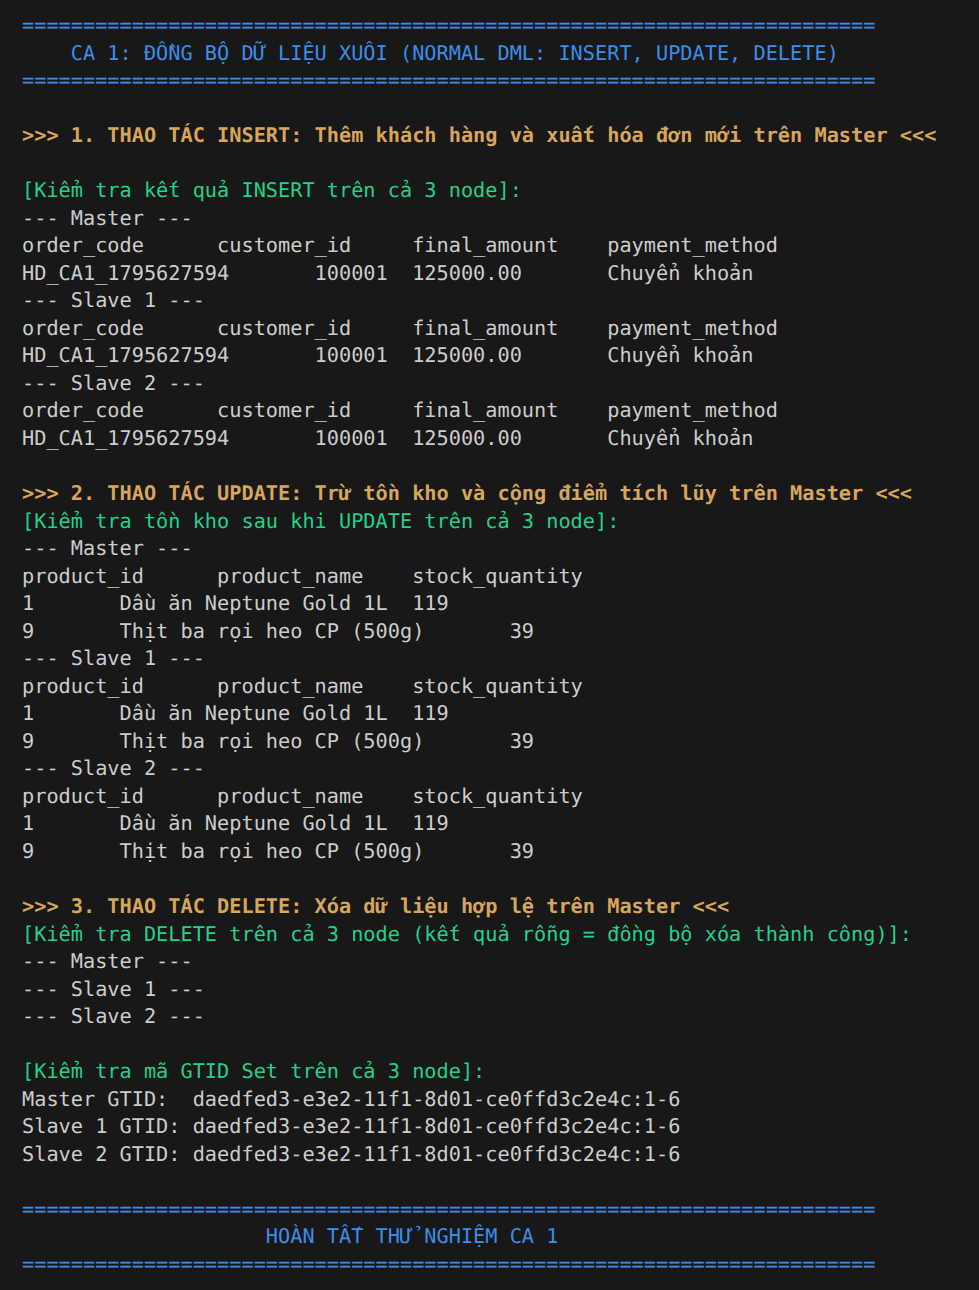
\includegraphics[width=0.92\textwidth,height=0.39\textheight,keepaspectratio]{images/ca1_dml.png}
    \caption{Ảnh chụp Terminal Ca 1: Đồng bộ hóa đơn, trừ tồn kho và xóa dữ liệu hợp lệ trên cả 3 Node}
    \label{fig:ca1}
\end{figure}

\clearpage
\section{Minh chứng Ca 2: Chặn ghi trái phép bằng Super Read-Only}
\begin{figure}[H]
    \centering
    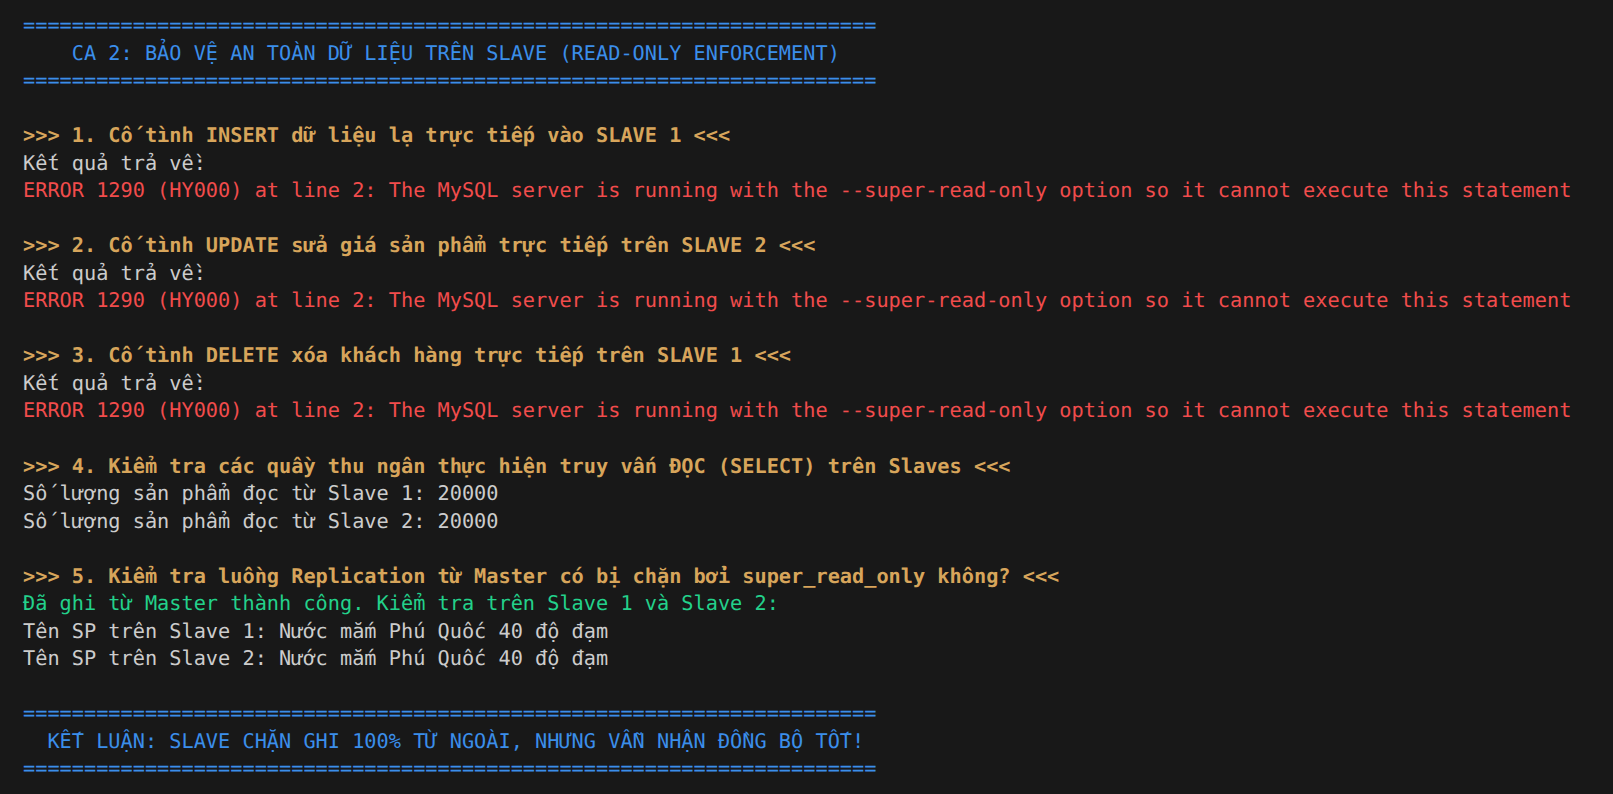
\includegraphics[width=0.95\textwidth,height=0.72\textheight,keepaspectratio]{images/ca2_readonly.png}
    \caption{Ảnh chụp Terminal Ca 2: Chặn các lệnh ghi trực tiếp bằng lỗi ERROR 1290 và đọc 20.000 sản phẩm trên Slave}
    \label{fig:ca2}
\end{figure}

\clearpage
\section{Minh chứng Ca 3: Gián đoạn mạng và tự động đồng bộ bù GTID}
\begin{figure}[H]
    \centering
    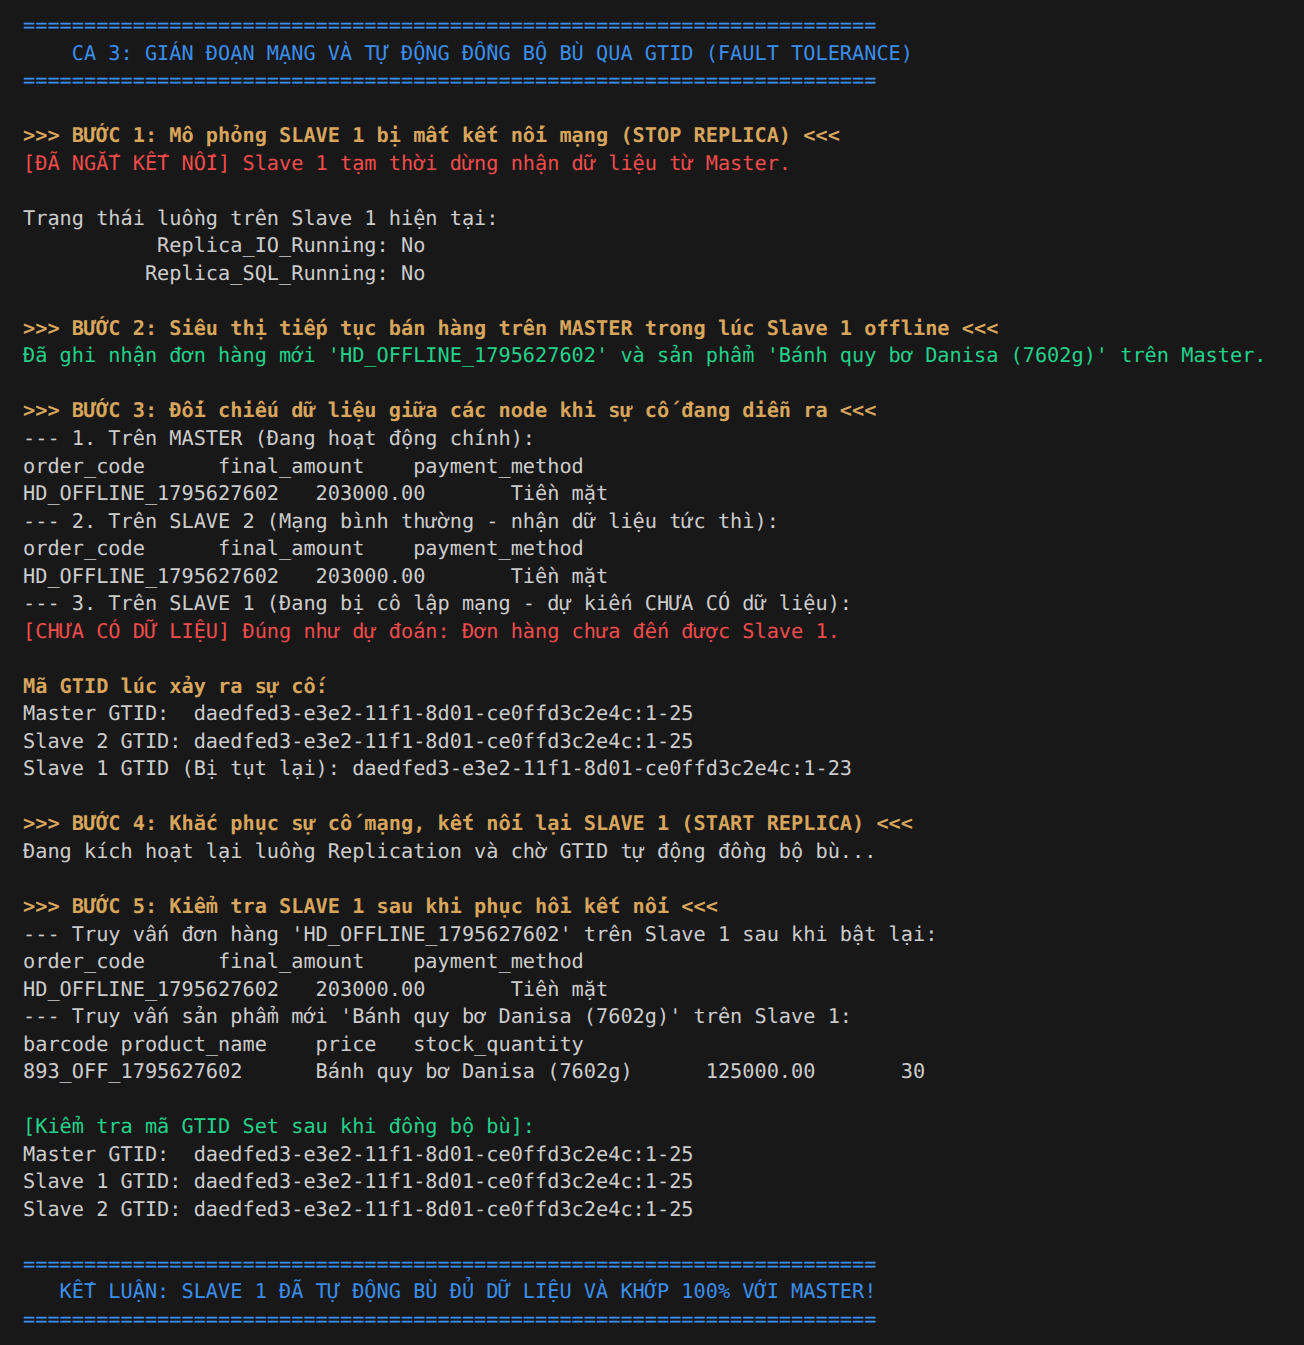
\includegraphics[width=0.92\textwidth,height=0.72\textheight,keepaspectratio]{images/ca3_fault_tolerance.png}
    \caption{Ảnh chụp Terminal Ca 3: Phục hồi kết nối Slave 1 và tự động kéo bù giao dịch qua GTID}
    \label{fig:ca3}
\end{figure}

\clearpage
\section{Minh chứng Ca 4: Đảm bảo tính toàn vẹn ACID và lệnh ROLLBACK}
\begin{figure}[H]
    \centering
    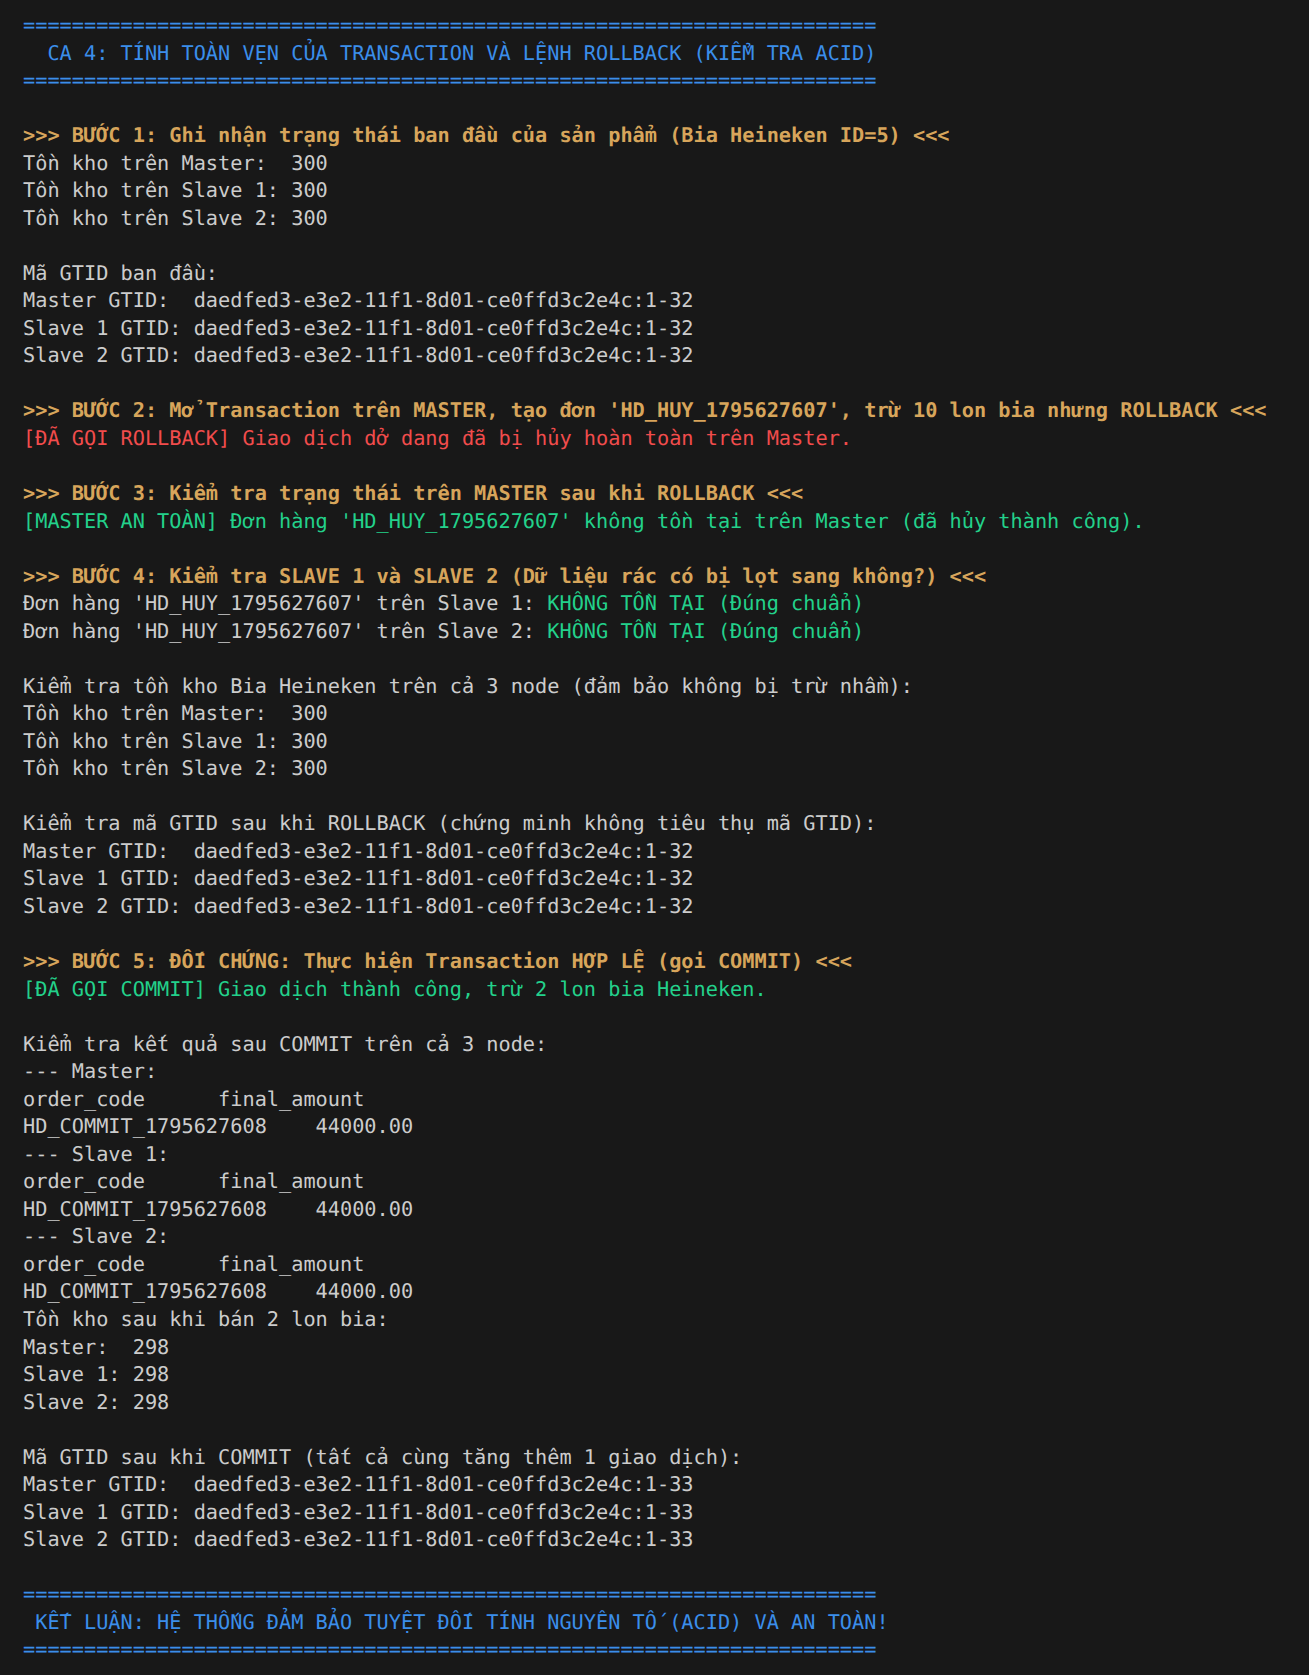
\includegraphics[width=0.92\textwidth,height=0.72\textheight,keepaspectratio]{images/ca4_rollback.png}
    \caption{Ảnh chụp Terminal Ca 4: Đối chứng giao dịch ROLLBACK không rò rỉ sang Slave và giao dịch COMMIT}
    \label{fig:ca4}
\end{figure}

\clearpage
\section{Minh chứng Ca 5: Nâng cấp cấu trúc bảng trực tuyến (Online DDL)}
\begin{figure}[H]
    \centering
    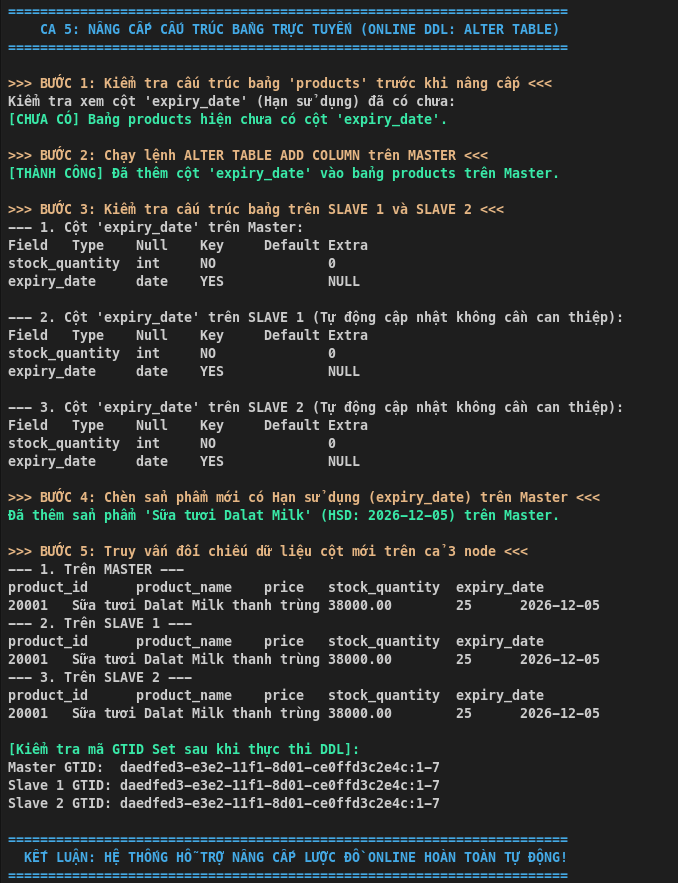
\includegraphics[width=0.92\textwidth,height=0.72\textheight,keepaspectratio]{images/ca5_online_ddl.png}
    \caption{Ảnh chụp Terminal Ca 5: Bổ sung cột \texttt{expiry\_date} trực tuyến và đồng bộ sang 2 Slave}
    \label{fig:ca5}
\end{figure}

\clearpage
\section{Minh chứng Ca 6: Đo lường độ trễ nhân bản dưới tải cao điểm}
\begin{figure}[H]
    \centering
    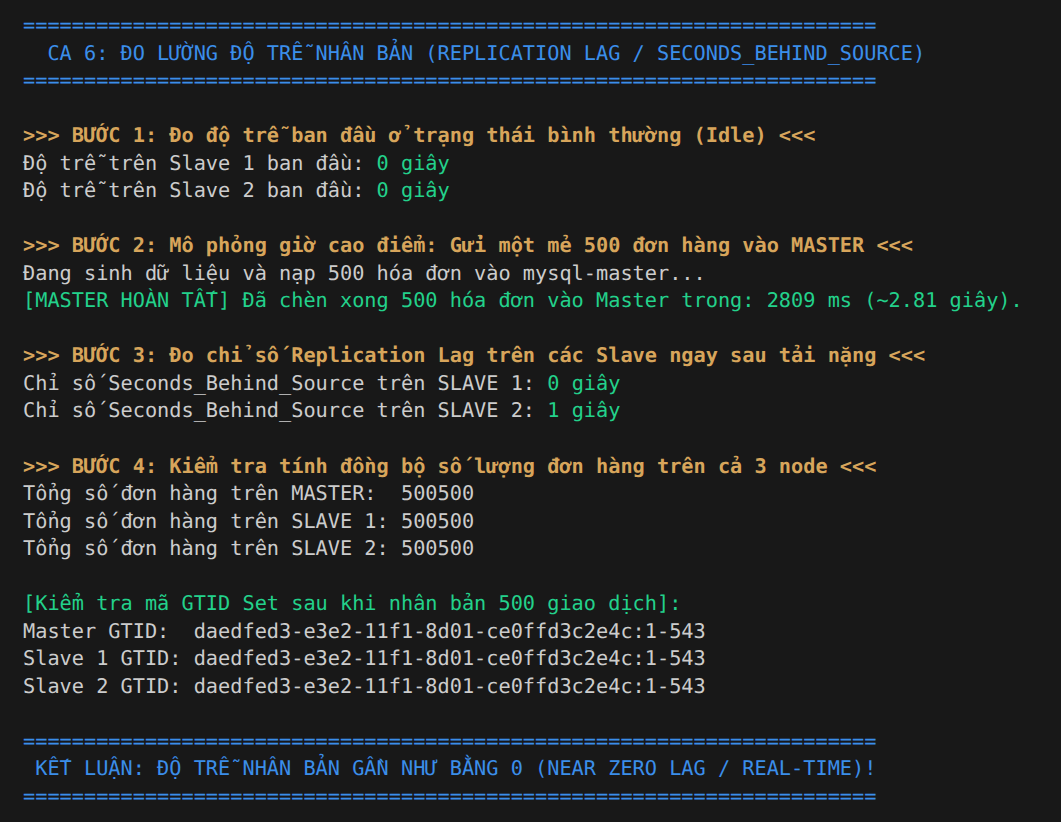
\includegraphics[width=0.92\textwidth,height=0.72\textheight,keepaspectratio]{images/ca6_replication_lag.png}
    \caption{Ảnh chụp Terminal Ca 6: Đo độ trễ \texttt{Seconds\_Behind\_Source} khi bơm 500 giao dịch liên tiếp}
    \label{fig:ca6}
\end{figure}

\clearpage
\section{Minh chứng Ca 7: Xử lý thảm họa sập Master (Manual Failover)}
\begin{figure}[H]
    \centering
    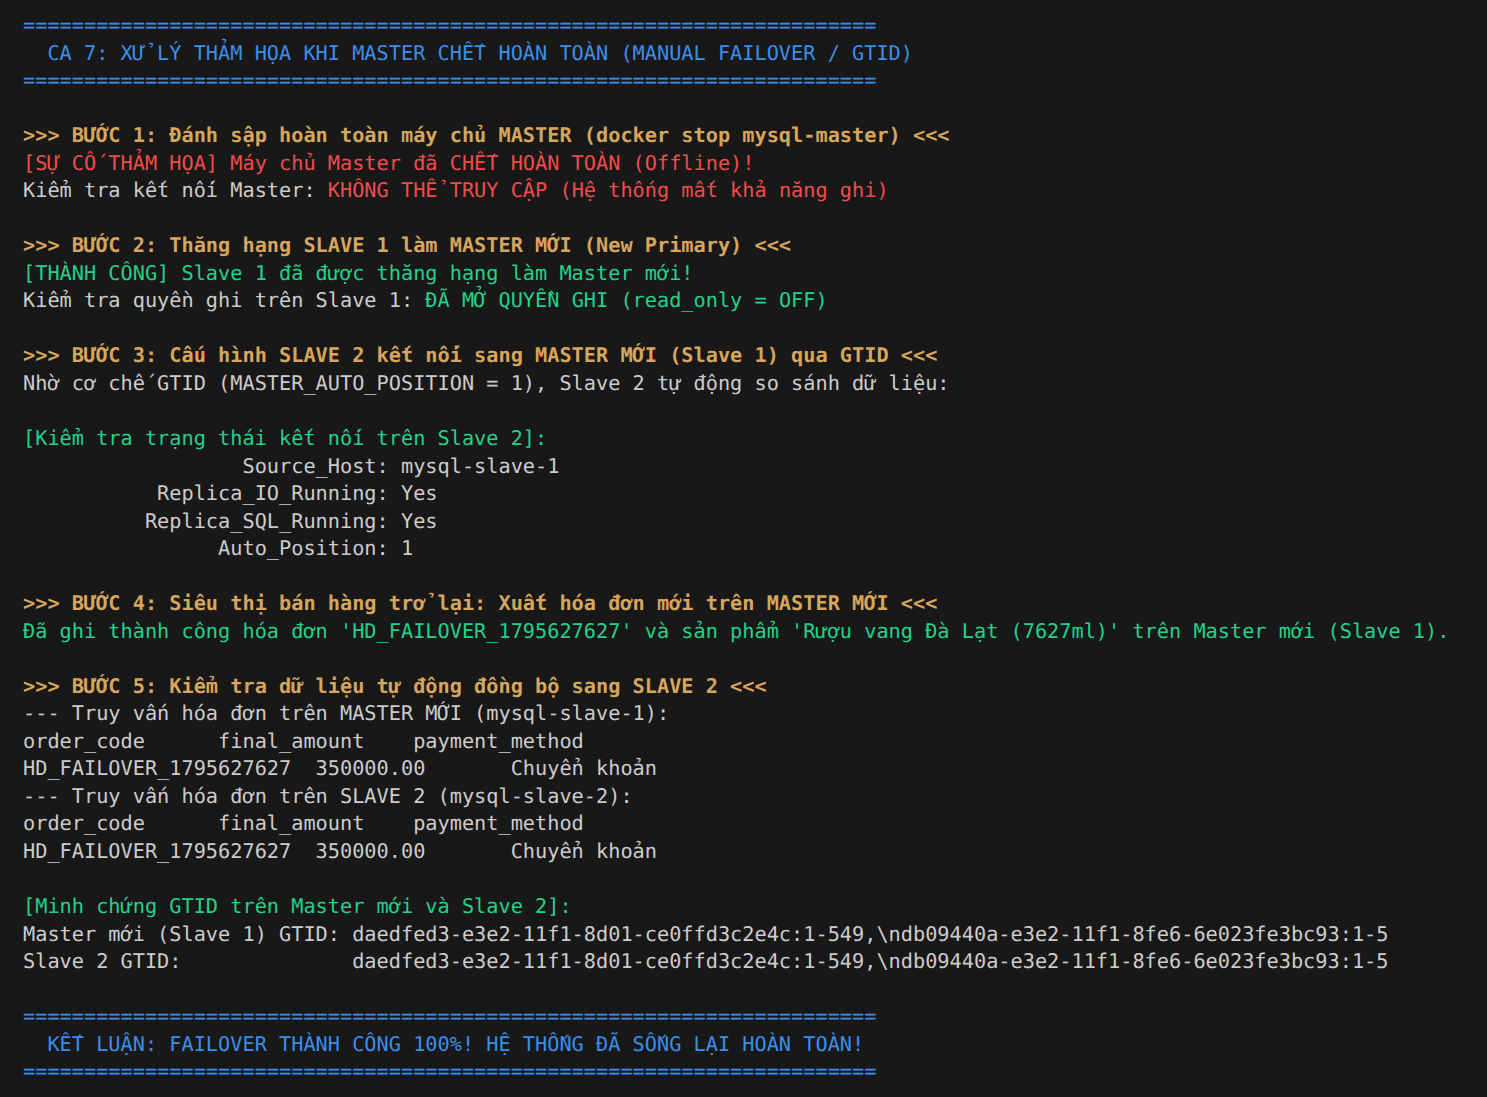
\includegraphics[width=0.95\textwidth,height=0.72\textheight,keepaspectratio]{images/ca7_failover.png}
    \caption{Ảnh chụp Terminal Ca 7: Thăng hạng Slave 1 làm Master mới và điều hướng lại Slave 2}
    \label{fig:ca7}
\end{figure}

\clearpage
\section{Minh chứng Ca 8: Đối soát 2,62 triệu bản ghi và hiệu năng truy vấn}
\begin{figure}[H]
    \centering
    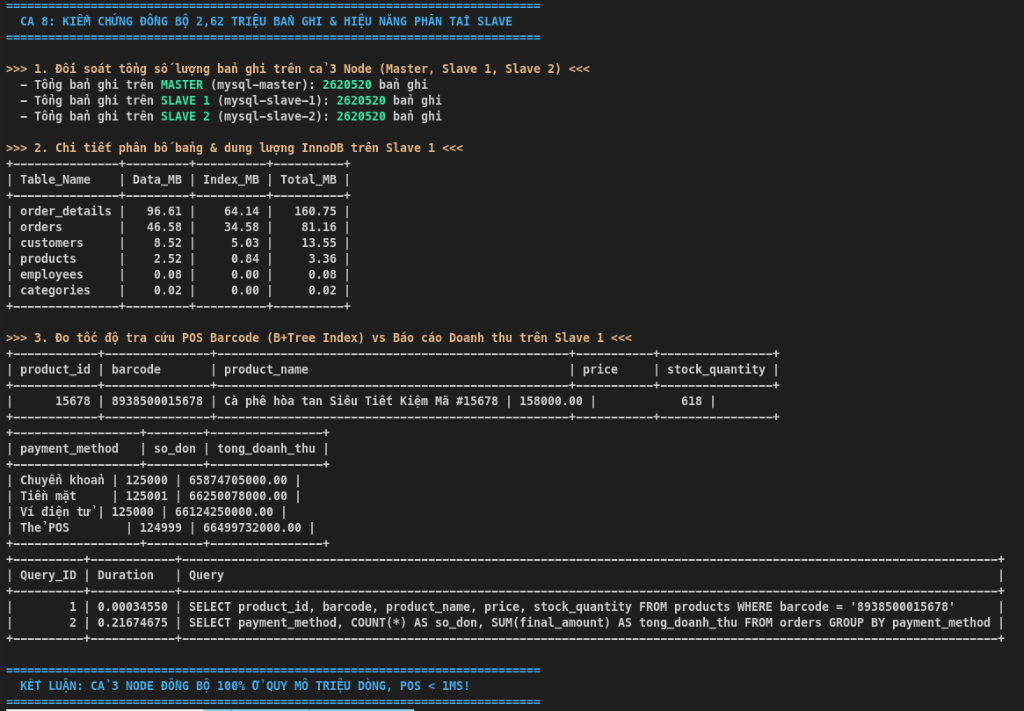
\includegraphics[width=0.95\textwidth,height=0.72\textheight,keepaspectratio]{images/ca8_million_scale.png}
    \caption{Ảnh chụp Terminal Ca 8: Đối soát 2.620.520 bản ghi/node và đo tốc độ truy vấn trên Slave}
    \label{fig:ca8}
\end{figure}

% ------------------------------------------------------------------------------
% PHỤ LỤC B: MÃ NGUỒN SQL KHỞI TẠO LƯỢC ĐỒ
% ------------------------------------------------------------------------------
\chapter{Mã Nguồn SQL Khởi Tạo Lược Đồ Và Dữ Liệu Nền}
\label{chap:appendix_sql}

Trong trường hợp người đọc muốn dựng thủ công cụm CSDL trực tiếp từ tệp báo cáo mà không tải từ kho lưu trữ GitHub, thực thi lần lượt hai khối mã SQL dưới đây trên \texttt{mysql-master} (sau khi đã hoàn tất các bước cấu hình tại Mục 3.1 -- 3.3) là có thể chạy thử ngay toàn bộ các kịch bản kiểm thử ở Chương 4.

\section{Khởi tạo lược đồ 6 bảng CSDL siêu thị}

\begin{lstlisting}[language=SQL, caption={Mã nguồn DDL khởi tạo CSDL và 6 bảng chuẩn InnoDB (tệp sql/01\_schema.sql)}]
CREATE DATABASE IF NOT EXISTS supermarket_db
  CHARACTER SET utf8mb4 COLLATE utf8mb4_unicode_ci;
USE supermarket_db;

DROP TABLE IF EXISTS order_details;
DROP TABLE IF EXISTS orders;
DROP TABLE IF EXISTS products;
DROP TABLE IF EXISTS customers;
DROP TABLE IF EXISTS employees;
DROP TABLE IF EXISTS categories;

CREATE TABLE categories (
    category_id INT AUTO_INCREMENT PRIMARY KEY,
    category_name VARCHAR(100) NOT NULL,
    description TEXT,
    created_at TIMESTAMP DEFAULT CURRENT_TIMESTAMP
) ENGINE=InnoDB DEFAULT CHARSET=utf8mb4 COLLATE=utf8mb4_unicode_ci;

CREATE TABLE products (
    product_id INT AUTO_INCREMENT PRIMARY KEY,
    barcode VARCHAR(50) UNIQUE NOT NULL,
    product_name VARCHAR(150) NOT NULL,
    category_id INT NOT NULL,
    unit VARCHAR(20) NOT NULL DEFAULT 'Cai',
    price DECIMAL(12, 2) NOT NULL,
    stock_quantity INT NOT NULL DEFAULT 0,
    created_at TIMESTAMP DEFAULT CURRENT_TIMESTAMP,
    CONSTRAINT fk_products_categories FOREIGN KEY (category_id)
      REFERENCES categories(category_id) ON DELETE RESTRICT ON UPDATE CASCADE
) ENGINE=InnoDB DEFAULT CHARSET=utf8mb4 COLLATE=utf8mb4_unicode_ci;

CREATE TABLE customers (
    customer_id INT AUTO_INCREMENT PRIMARY KEY,
    customer_name VARCHAR(100) NOT NULL,
    phone VARCHAR(15) UNIQUE,
    membership_card VARCHAR(30) UNIQUE,
    points INT DEFAULT 0,
    created_at TIMESTAMP DEFAULT CURRENT_TIMESTAMP
) ENGINE=InnoDB DEFAULT CHARSET=utf8mb4 COLLATE=utf8mb4_unicode_ci;

CREATE TABLE employees (
    employee_id INT AUTO_INCREMENT PRIMARY KEY,
    employee_name VARCHAR(100) NOT NULL,
    role VARCHAR(50) DEFAULT 'Thu ngan',
    phone VARCHAR(15),
    salary DECIMAL(12, 2) DEFAULT 0,
    created_at TIMESTAMP DEFAULT CURRENT_TIMESTAMP
) ENGINE=InnoDB DEFAULT CHARSET=utf8mb4 COLLATE=utf8mb4_unicode_ci;

CREATE TABLE orders (
    order_id INT AUTO_INCREMENT PRIMARY KEY,
    order_code VARCHAR(30) UNIQUE NOT NULL,
    customer_id INT NULL,
    employee_id INT NOT NULL,
    total_amount DECIMAL(12, 2) NOT NULL DEFAULT 0,
    discount_amount DECIMAL(12, 2) DEFAULT 0,
    final_amount DECIMAL(12, 2) NOT NULL DEFAULT 0,
    payment_method VARCHAR(30) DEFAULT 'Tien mat',
    order_date TIMESTAMP DEFAULT CURRENT_TIMESTAMP,
    CONSTRAINT fk_orders_customers FOREIGN KEY (customer_id)
      REFERENCES customers(customer_id) ON DELETE SET NULL ON UPDATE CASCADE,
    CONSTRAINT fk_orders_employees FOREIGN KEY (employee_id)
      REFERENCES employees(employee_id) ON DELETE RESTRICT ON UPDATE CASCADE
) ENGINE=InnoDB DEFAULT CHARSET=utf8mb4 COLLATE=utf8mb4_unicode_ci;

CREATE TABLE order_details (
    order_detail_id INT AUTO_INCREMENT PRIMARY KEY,
    order_id INT NOT NULL,
    product_id INT NOT NULL,
    quantity INT NOT NULL,
    unit_price DECIMAL(12, 2) NOT NULL,
    subtotal DECIMAL(12, 2) NOT NULL,
    CONSTRAINT fk_order_details_orders FOREIGN KEY (order_id)
      REFERENCES orders(order_id) ON DELETE CASCADE ON UPDATE CASCADE,
    CONSTRAINT fk_order_details_products FOREIGN KEY (product_id)
      REFERENCES products(product_id) ON DELETE RESTRICT ON UPDATE CASCADE
) ENGINE=InnoDB DEFAULT CHARSET=utf8mb4 COLLATE=utf8mb4_unicode_ci;
\end{lstlisting}

\clearpage
\section{Dữ liệu nền phục vụ kiểm thử độc lập}

\begin{lstlisting}[language=SQL, caption={Nạp các bản ghi danh mục và mặt hàng gốc phục vụ kiểm thử (tệp sql/02\_sample\_data.sql)}]
USE supermarket_db;

INSERT INTO categories (category_name, description) VALUES
('Thuc pham tuoi song', 'Thit, ca, hai san, rau cu'),
('Hoa my pham', 'Xa phong, nuoc giat, dau goi'),
('Banh keo', 'Banh ngot, snack, keo'),
('Do uong', 'Nuoc ngot, nuoc khoang, sua, bia'),
('Gia vi & Do kho', 'Nuoc mam, dau an, gao');

INSERT INTO employees (employee_name, role, phone, salary) VALUES
('Nguyen Van An', 'Thu ngan', '0901234567', 7500000),
('Tran Thi Bich', 'Thu ngan', '0912345678', 7500000),
('Le Hoang Nam', 'Quan ly ca', '0987654321', 12000000);

INSERT INTO customers (customer_name, phone, membership_card, points) VALUES
('Pham Minh Tuan', '0933112233', 'VIP001', 150),
('Vu Thi Mai', '0944223344', 'MEM002', 45),
('Dang Quoc Huy', '0977889900', 'MEM003', 80);

INSERT INTO products (barcode, product_name, category_id, unit, price, stock_quantity) VALUES
('893456701', 'Dau an Neptune Gold 1L', 5, 'Chai', 52000, 120),
('893456702', 'Nuoc mam Nam Ngu 750ml', 5, 'Chai', 38000, 200),
('893456703', 'Gao ST25 tui 5kg', 5, 'Tui', 185000, 50),
('893456704', 'Nuoc ngot Coca Cola 320ml', 4, 'Lon', 10000, 500),
('893456705', 'Bia Heineken lon 330ml', 4, 'Lon', 22000, 300),
('893456706', 'Snack khoai tay OStar', 3, 'Goi', 14000, 150),
('893456707', 'Nuoc giat OMO Matic 2kg', 2, 'Tui', 145000, 80),
('893456708', 'Dau goi Clear Men 630g', 2, 'Chai', 179000, 60),
('893456709', 'Thit ba roi heo CP (500g)', 1, 'Hop', 75000, 40),
('893456710', 'Bap cai trang Da Lat (kg)', 1, 'Kg', 18000, 100);
\end{lstlisting}

\end{document}
